\chapter{Results}
\label{cap:results}

In accordance with the OpenUP lifecycle described in chapter~\ref{cap:methodology}, the following subsections will detail the development phases of the first version of FENCE, emphasizing the results of each phase and thoroughly explaining the decisions made in the design and development of the tool.

\section{Inception phase}

In this first phase, initial meetings with stakeholders took place, where a first contact was established and from which the project objectives would begin to be defined. The idea of the preliminary project was consolidated, and the functionalities and design of FENCE began to be roughly sketched out.

Therefore, this meetings with the stakeholders, Aurora Vizcaíno and José Ángel Olivas, focused on defining, on the one hand, the basic functionalities of the tool (STC measurement, dashboard features, settings and preferences) and, on the other hand, the features that would make FENCE an innovative tool (use of fuzzy inference system to improve STC measurement or a recommending system aimed to enhance STC levels). These features were conveniently formalized as requirements, as we will see in the elaboration phase.

As previously mentioned, the initiation phase in OpenUP involves the definition of the roles of the different stakeholders. In this case, it was decided that Aurora Vizcaíno would supervise the development of the application in general terms, while José Ángel Olivas would monitor the part of the system related to the intensification competencies, such as the implementation of the expert system or the introduction of fuzzy logic into the system.

Moreover, from a technical point of view, it was also agreed that FENCE would be a web application capable of offering services locally and, if possible, online. Furthermore, ideas also began to be sketched out on what the web application would graphically look like, as shown in the sketches represented in Figure~\ref{fig:dash_mockup} and Figure~\ref{fig:rec_mockup}.

\begin{figure}
	\centering
	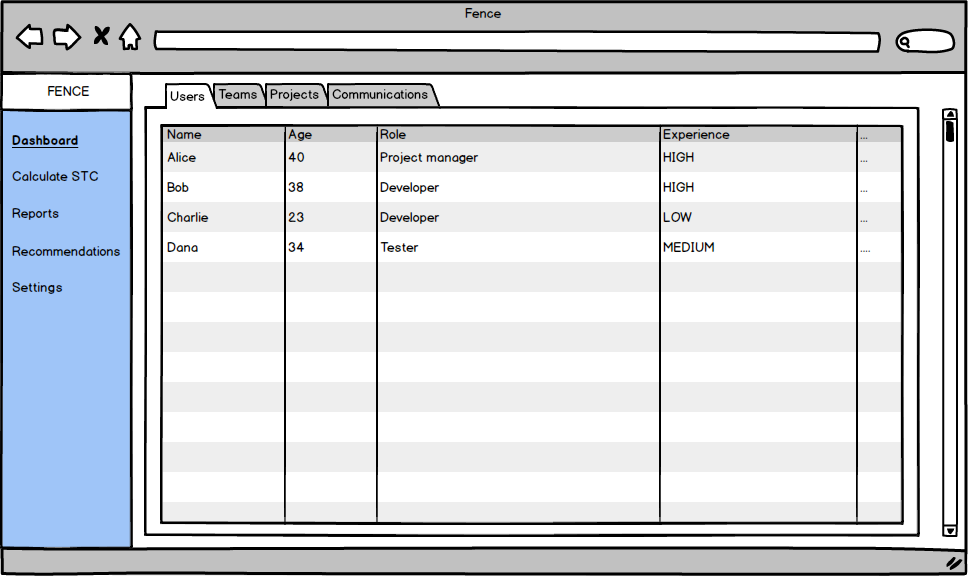
\includegraphics[width=0.9\linewidth]{4_mockup-dashboard}
	\caption[Dashboard mockup]{Dashboard mockup}
	\label{fig:dash_mockup}
\end{figure}

\begin{figure}
	\centering
	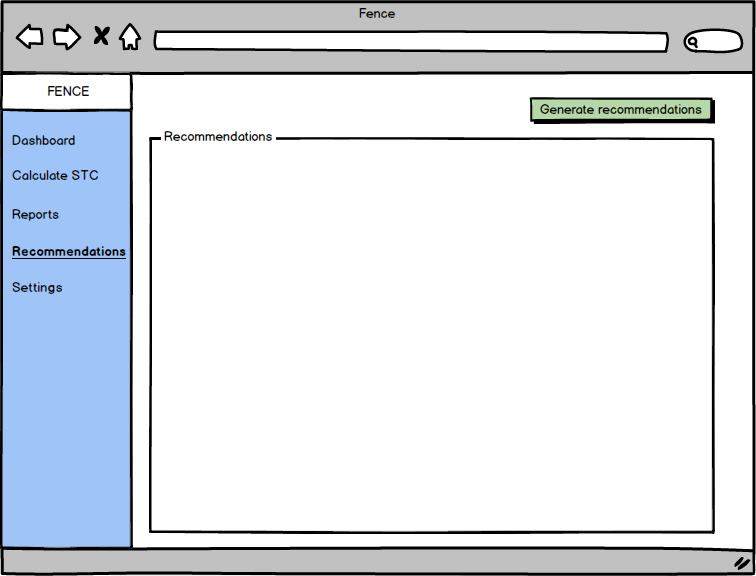
\includegraphics[width=0.9\linewidth]{4_mockup-recommendations}
	\caption[Recommendations window mockup]{Recommendations window mockup}
	\label{fig:rec_mockup}
\end{figure}

With clear objectives and an approximate and viable idea of the project to be undertaken, we proceeded to the elaboration phase, where these objectives and requirements would be formalized thus establishing the foundations of FENCE.

\section{Elaboration phase}

Initially, the objectives pursued in this phase are the formalization of the system requirements, the decision on the architecture to be used, as well as its design and data model. On this basis, it would be possible to establish a project planning, as well as a cost estimation adjusted to the development time and resources used.

Moreover, some key learning aspects were carried out at this stage, such as training in the Spring framework or MongoDB. Thus, further research in these technologies in the early project stages would facilitate future work and ensure more consistent progress.

\subsection{Requirements}

The requirements elicitation is the process in which the description of the properties that the system to be developed must meet is performed. These features are expressed by the client, while the interviewer is in charge of collecting the necessary information and expressing it in a precise and unambiguous document.

In the case of this project, the process of requirements elicitation was carried out following the structured interview method, as detailed in \cite{toro_metodologia_2000}. These interviews are divided in three phases: preparation, realization and analysis, and they are a close and direct way to directly understand interests of the stakeholders. Therefore, the interview was approached as follows:

\begin{itemize}
	\item First the questions to be asked were decided, a structured script was drawn up with the questions to be asked and the order to be followed.
	\item Subsequently, a first meeting was held with the main stakeholder, Aurora Vizcaíno, where the functional and non-functional requirements of the tool were broadly agreed upon.
	\item Regular follow-up meetings would be held throughout the project, where these requirements would be not only evaluated but also adjusted to suggested changes and improvements.
\end{itemize}

The initial requirements were expressed in precise and unambiguous language, as will be shown in the following subsections. Thus, after their validation by the client, the use cases and modelling of FENCE would proceed.

\subsubsection{FUNCTIONAL REQUIREMENTS}

Functional requirements represent which functionalities should be covered by the system to be developed, considering inputs and outputs as well as the behaviour of the software. After the interviews with stakeholders, these functional requirements were agreed upon and duly expressed, giving rise to the set of functionalities represented in Table~\ref{tb:funct-req}.

\begin{table}
	\centering
	\caption[Functional requirements]{Functional requirements}
	\label{tb:funct-req}
	\resizebox{\textwidth}{!}{%
	\begin{tabular}{|c|c|l|c|}
	\hline
	\textbf{ID} &
	  \textbf{Description} &
	  \multicolumn{1}{c|}{\textbf{Objectives}} &
	  \textbf{Priority} \\ \hline\hline
	\textit{FR1} &
	  Users STC measurement &
	  \begin{tabular}[c]{@{}l@{}}The tool must calculate and display  the STC \\ levels of the users in the organization.\end{tabular} &
	  High \\ \hline
	\textit{FR2} &
	  Teams STC measurement &
	  \begin{tabular}[c]{@{}l@{}}The tool must calculate and display the STC \\ levels of the teams in the organization.\end{tabular} &
	  High \\ \hline
	\textit{FR3} &
	  Projects STC measurement &
	  \begin{tabular}[c]{@{}l@{}}The tool must calculate the STC \\ levels of the projects in the organization.\end{tabular} &
	  High \\ \hline
	\textit{FR4} &
	  Recommendations &
	  \begin{tabular}[c]{@{}l@{}}The system must provide recommendations \\ based on the existing coordination gaps to improve \\ the STC levels of the organization.\end{tabular} &
	  High \\ \hline
	\textit{FR5} &
	  Dashboard: employees &
	  \begin{tabular}[c]{@{}l@{}}The tool should allow to perform CRUD \\ operations over employees as resources.\end{tabular} &
	  Medium \\ \hline
	\textit{FR6} &
	  Dashboard: teams &
	  \begin{tabular}[c]{@{}l@{}}The tool should allow to perform CRUD\\ operations over teams as resources.\end{tabular} &
	  Medium \\ \hline
	\textit{FR7} &
	  Dashboard: projects &
	  \begin{tabular}[c]{@{}l@{}}The tool should allow to perform CRUD \\ operations over  projects as resources.\end{tabular} &
	  Medium \\ \hline
	\textit{FR8} &
	  Dashboard: tasks &
	  \begin{tabular}[c]{@{}l@{}}The tool should allow to perform CRUD \\ operations over tasks as resources.\end{tabular} &
	  Medium \\ \hline
	\textit{FR9} &
	  Dashboard: task assignments &
	  \begin{tabular}[c]{@{}l@{}}The tool should allow to perform CRUD \\ operations over tasks assignments as resources.\end{tabular} &
	  Medium \\ \hline
	\textit{FR10} &
	  Dashboard: task dependencies &
	  \begin{tabular}[c]{@{}l@{}}The tool should allow to perform CRUD \\ operations over tasks dependencies as resources.\end{tabular} &
	  Medium \\ \hline
	\textit{FR11} &
	  Dashboards: communications &
	  \begin{tabular}[c]{@{}l@{}}The tool should allow to visualize \\ communications within the organization.\end{tabular} &
	  Medium \\ \hline
	\textit{FR12} &
	  Users STC visualization &
	  \begin{tabular}[c]{@{}l@{}}The tool should display visual information \\ about the users' STC levels along time.\end{tabular} &
	  Medium \\ \hline
	\textit{FR13} &
	  Teams STC visualization &
	  \begin{tabular}[c]{@{}l@{}}The tool should display visual information \\ about the teams’ STC levels along time.\end{tabular} &
	  Medium \\ \hline
	\textit{FR14} &
	  Projects STC visualization &
	  \begin{tabular}[c]{@{}l@{}}The tool should display visual information \\ about the projects' STC levels along time.\end{tabular} &
	  Medium \\ \hline
	\textit{FR15} &
	  Custom project‘s lack of coordination threshold &
	  \begin{tabular}[c]{@{}l@{}}The tool will allow to customize from which \\ threshold of lack of coordination recommendations \\ should be provided for a given project.\end{tabular} &
	  Low \\ \hline
	\textit{FR16} &
	  Custom users’ lack of coordination threshold &
	  \begin{tabular}[c]{@{}l@{}}The tool will allow to customize from which \\ threshold of lack of coordination recommendations \\ should be provided for a given pair of employees \\ within a project.\end{tabular} &
	  Low \\ \hline
	\end{tabular}%
	}
\end{table}

\subsubsection{NON FUNCTIONAL REQUIREMENTS}

Non-functional requirements are complemented by functional requirements to fully define the expected characteristics of the system. These requirements focus on representing quality and technical features as well as conditions and constraints expressed by the customer. Thus, the non-functional requirements for this project are shown in the Table~\ref{tb:nonfunc-req}.

\begin{table}
	\centering
	\caption{Non-functional requirements}
	\label{tb:nonfunc-req}
	\resizebox{\textwidth}{!}{%
	\begin{tabular}{|c|c|l|c|}
	\hline
	\textbf{ID} &
	  \textbf{Description} &
	  \multicolumn{1}{c|}{\textbf{Objectives}} &
	  \textbf{Type} \\ \hline\hline
	\textit{NFR1} &
	  Labels &
	  \begin{tabular}[c]{@{}l@{}}Linguistic labels will be used to represent ambiguous terms,   \\ such as user experience, English level, or dependency weight \\ between tasks.\end{tabular} &
	  Usability \\ \hline
	\textit{NFR2} &
	  Web application &
	  \begin{tabular}[c]{@{}l@{}}The application will be deployed as a web service, preferably  \\  at a local level, but with the possibility of public offering.\end{tabular} &
	  Usability \\ \hline
	\textit{NFR3} &
	  Browser compatibility &
	  \begin{tabular}[c]{@{}l@{}}The application must be able to run on desktop devices using   \\ conventional browsers such as Google Chrome or Mozilla Firefox.\end{tabular} &
	  Compatibility \\ \hline
	\textit{NFR4} &
	  Cloud database &
	  \begin{tabular}[c]{@{}l@{}}A database management system available in the cloud will be   \\ used, in order to facilitate the integration of the tool with remote systems.\end{tabular} &
	  Compatibility \\ \hline
	\textit{NFR5} &
	  Performance &
	  \begin{tabular}[c]{@{}l@{}}The application will run fluently in the interaction with   \\ its different components, offering an adequate performance and user  \\  experience.\end{tabular} &
	  Performance \\ \hline
	\end{tabular}%
	}
\end{table}

\subsection{Use cases and modules}

Once the system requirements had been compiled, the definition of the use cases was undertaken. The use case model is shown in Figure~\ref{fig:cdu-model}, which represents the activities carried out by the entities (actors) according to the expected system functionalities.

\begin{figure}
	\centering
	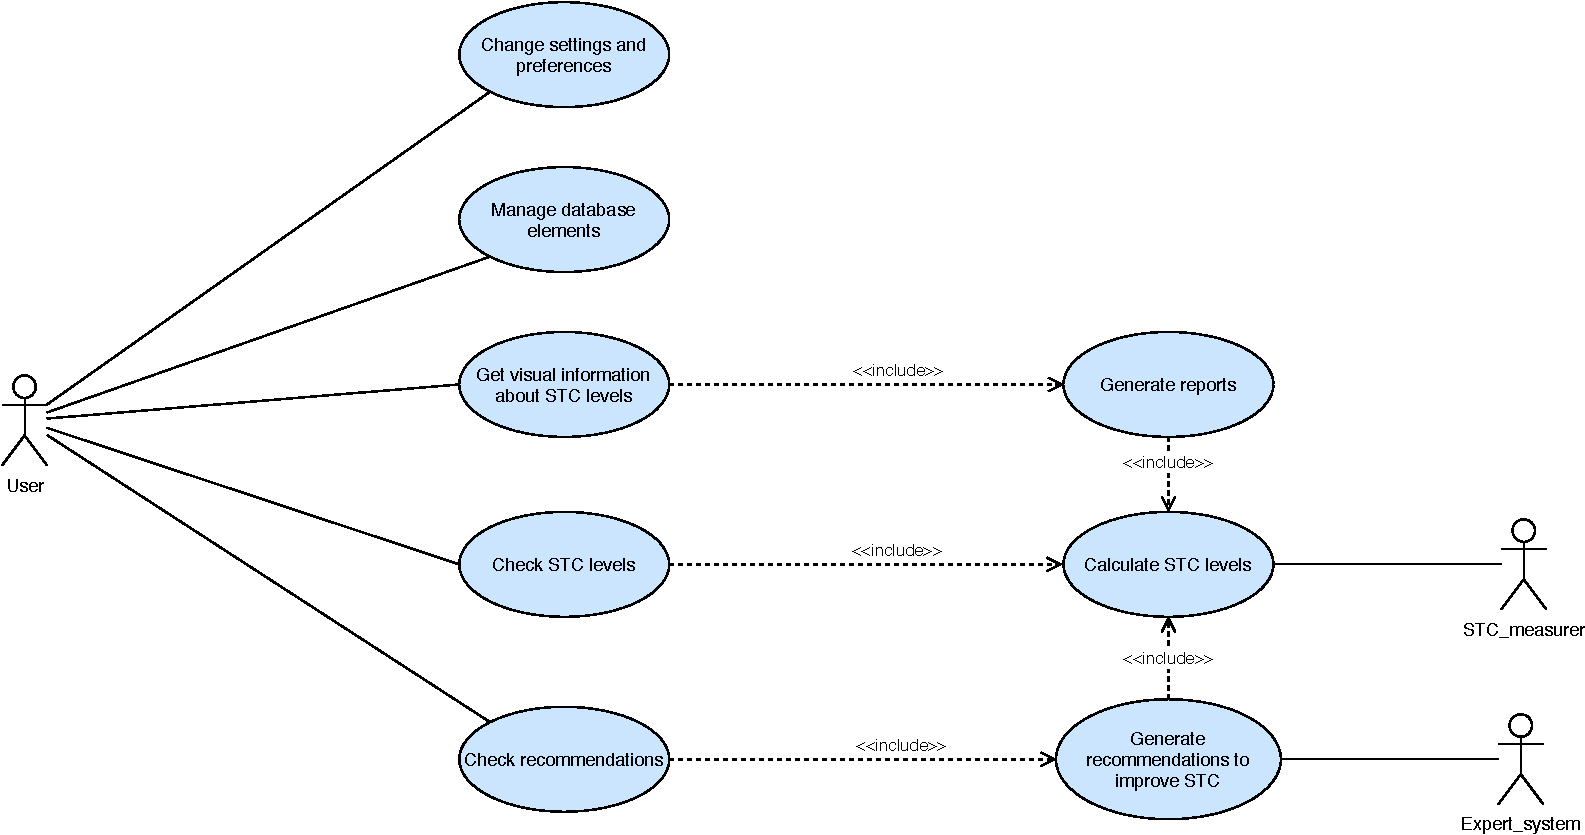
\includegraphics[width=0.95\linewidth]{4_cdu-diagram}
	\caption[Use cases model]{Use cases model}
	\label{fig:cdu-model}
\end{figure}

Once the use cases were identified, they were grouped into different functional modules in order to organize the development of the subsystems that compose the application. These are listed in Table~\ref{tb:func-mod}, together with their definitions and priority levels.

\begin{table}
	\centering
	\caption{Functional modules}
	\label{tb:func-mod}
	\resizebox{\textwidth}{!}{%
	\begin{tabular}{|c|c|l|c|}
	\hline
	\textbf{ID} &
	  \textbf{Module description} &
	  \multicolumn{1}{c|}{\textbf{Objectives}} &
	  \textbf{Priority} \\ \hline\hline
	\textit{M1} &
	  API skeleton &
	  \begin{tabular}[c]{@{}l@{}}Development of the application skeleton, creation of the API   \\ resources as well as connection and operations on the database.\end{tabular} &
	  High \\ \hline
	\textit{M2} &
	  Main  user interface &
	  \begin{tabular}[c]{@{}l@{}}Implementation of the dashboard functionalities and   \\ elaboration of the main windows of the web application.\end{tabular} &
	  High \\ \hline
	\textit{M3} &
	  STC measurement &
	  \begin{tabular}[c]{@{}l@{}}Extraction of assignments, dependencies, and current   \\ coordination, as well as coordination requirements and gaps. \\ Computation of STC at employees, teams, and projects levels.\end{tabular} &
	  High \\ \hline
	\textit{M4} &
	  Data visualization &
	  \begin{tabular}[c]{@{}l@{}}Graphic representation of the STC levels history, allowing   \\ to see comparisons and the variation of these levels along time.\end{tabular} &
	  Medium \\ \hline
	\textit{M5} &
	  Recommendation system &
	  \begin{tabular}[c]{@{}l@{}}System for the detection of coordination gaps and   \\ recommendation of solutions to improve the levels \\ of STC based on expert knowledge.\end{tabular} &
	  Medium \\ \hline
	\textit{M6} &
	  Settings and preferences &
	  Customization and tool settings configuration. &
	  Low \\ \hline
	\end{tabular}%
	}
\end{table}

The decomposition of the application in functional modules would facilitate the way to proceed in the construction phase of the life cycle, performing micro-increments that could be tested and evaluated by the stakeholders. This modular division would also facilitate the planning and estimation of development times, as it will be seen in the following sub-section.

\subsection{Planification}

Having identified the functionalities to be implemented and the general project decomposition, it was divided into the iterations shown in Table~\ref{tb:proj-iters}. Each one, with an estimated duration, would represent an evaluable and revisable micro-increment of the application.

\begin{table}
	\centering
	\caption{Project iterations}
	\label{tb:proj-iters}
	\begin{tabular}{|c|l|c|}
	\hline
	\textbf{Iteration} &
	  \multicolumn{1}{c|}{\textbf{Summary}} &
	  \textbf{Estimated time} \\ \hline\hline
	\textit{IT0} &
	  \begin{tabular}[c]{@{}l@{}}Definition of general objectives, first draft and   \\ preliminary meetings.\end{tabular} &
	  1 week \\ \hline
	\textit{IT1} &
	  \begin{tabular}[c]{@{}l@{}}Planning, requirements elicitation, role assignment, \\ usecase modelling and design.\end{tabular} &
	  2 weeks \\ \hline
	\textit{IT2} & Module 1 implementation             & 1 week  \\ \hline
	\textit{IT3} & Module 2 implementation             & 2 weeks \\ \hline
	\textit{IT4} & Module 3 implementation             & 4 weeks \\ \hline
	\textit{IT5} & Module 4 implementation             & 1 week  \\ \hline
	\textit{IT6} & Module 5 implementation             & 3 weeks \\ \hline
	\textit{IT7} & Module 6 implementation             & 1 week  \\ \hline
	\textit{IT8} & Documentation, tests and deployment & 3 weeks \\ \hline
	\textit{IT9} & Review and submission preparation   & 2 weeks \\ \hline
	\end{tabular}
\end{table}

Based on these iterations, the project schedule was established (see Table~\ref{tb:schedule}). This was largely achieved, apart from some slight fluctuations which did not affect the project, as they were due to improvements in the different functional modules, rather than delays.

\begin{table}
	\centering
	\caption{Project scheduling}
	\label{tb:schedule}
	\resizebox{\textwidth}{!}{%
	\begin{tabular}{|c|c|c|c|c|c|c|c|c|c|}
	\hline
	\textbf{Inception phase} &
	  \textbf{Elaboration phase} &
	  \multicolumn{6}{c|}{\textbf{Construction phase}} &
	  \multicolumn{2}{c|}{\textbf{Transition phase}} \\ \hline\hline
	\textit{IT0} &
	  \textit{IT1} &
	  \textit{IT2} &
	  \textit{IT3} &
	  \textit{IT4} &
	  \textit{IT5} &
	  \textit{IT6} &
	  \textit{IT7} &
	  \textit{IT8} &
	  \textit{IT9} \\ \hline
	\begin{tabular}[c]{@{}c@{}}From: 7th \\ January\\  -   \\ To: 31st\\  January\end{tabular} &
	  \begin{tabular}[c]{@{}c@{}}From: 1st \\ February\\ -  \\ To: 15th \\ February\end{tabular} &
	  \begin{tabular}[c]{@{}c@{}}From: 16th \\ February\\   -  \\    To: 23th \\ February\end{tabular} &
	  \begin{tabular}[c]{@{}c@{}}From: 24th\\  February\\   -  \\ To: 8th\\ March\end{tabular} &
	  \begin{tabular}[c]{@{}c@{}}From: 9th \\ March\\   -    \\ To: 5th\\ April\end{tabular} &
	  \begin{tabular}[c]{@{}c@{}}From: 6th \\ April\\   -  \\    To: 12th \\ April\end{tabular} &
	  \begin{tabular}[c]{@{}c@{}}From: 13th \\ April\\  -   \\    To: 3rd \\ May\end{tabular} &
	  \begin{tabular}[c]{@{}c@{}}From: 4th \\ May\\  -   \\    To: 10th \\ May\end{tabular} &
	  \begin{tabular}[c]{@{}c@{}}From: 11th \\ May\\   -  \\    To: 31st \\ May\end{tabular} &
	  \begin{tabular}[c]{@{}c@{}}From: 1st \\ June\\  -  \\    To: 14th \\ June\end{tabular} \\ \hline
	1 week &
	  2 weeks &
	  1 week &
	  2 weeks &
	  4 weeks &
	  1 week &
	  3 weeks &
	  1 week &
	  3 weeks &
	  2 weeks \\ \hline
	1 week &
	  2 weeks &
	  \multicolumn{6}{c|}{12 weeks} &
	  \multicolumn{2}{c|}{3 weeks} \\ \hline
	\multicolumn{10}{|c|}{\textbf{Total: 18 weeks}} \\ \hline
	\end{tabular}%
	}
\end{table}

\subsection{Cost estimation}

In this section, the cost estimation of the project, calculated from the working time and resources used, is broken down. For this estimation, the variables shown in Table~\ref{tb:costs} have been considered, giving rise to the total cost of 7206.6 €.

\begin{table}
	\centering
	\caption{Project cost estimation}
	\label{tb:costs}
	\begin{tabular}{c|c|}
	\hline
	\multicolumn{1}{|c|}{\textbf{Variable}}   & \textbf{Value}                      \\ \hline\hline
	\multicolumn{1}{|c|}{Total working hours} & $\approx$ 630 hours $*$ 11,22 €/hour = 7068 € \\ \hline
	\multicolumn{1}{|c|}{\begin{tabular}[c]{@{}c@{}}Indirect investments \\ (resources, electricity consume, etc.)\end{tabular}} & 138.6   € \\ \hline
	                                          & 7206.6   €                          \\ \cline{2-2} 
	\end{tabular}%
	
\end{table}

The salary per hour of the analyst-programmer is reflected in \cite{tecnoempleo}, with data updated up to May 2020. At the same time, the price of software resources has been omitted because only free software or software covered by academic licenses has been used.

\subsection{Architecture and design}

The elaboration phase of the OpenUp lifecycle includes the selection of the architecture to be employed. So, at this stage it was decided that FENCE would be a client-server application based on a layered architecture, whose characteristics are described below. The choice of client-server as the architecture of FENCE was agreed in order to be able to deploy the tool as a web service if necessary. In this way, this would be a portable application, which would allow the user to run the tool from any browser without the need for additional software.

Moreover, a preliminary data model was also established, establishing the main collections and documents that would comprise it, as well as their attributes and possible relationships.

\subsubsection{LAYERED ARCHITECTURE}

Layer-based architecture \cite{layered_architecture} is one of the most common design patterns in the development of client-server web applications. In this type of architecture, the different modules that comprise the system (layers) are organized horizontally, so that each layer of the application fulfils a specific role.

Spring Boot \cite{spring_boot} provides a great simplicity when implementing this type of RESTful layered services \cite{api_rest},  so it is on this basis on which the FENCE architecture is based (see Figure~\ref{fig:layer_arch} and Figure~\ref{fig:layers-sample}):

\begin{figure}
	\centering
	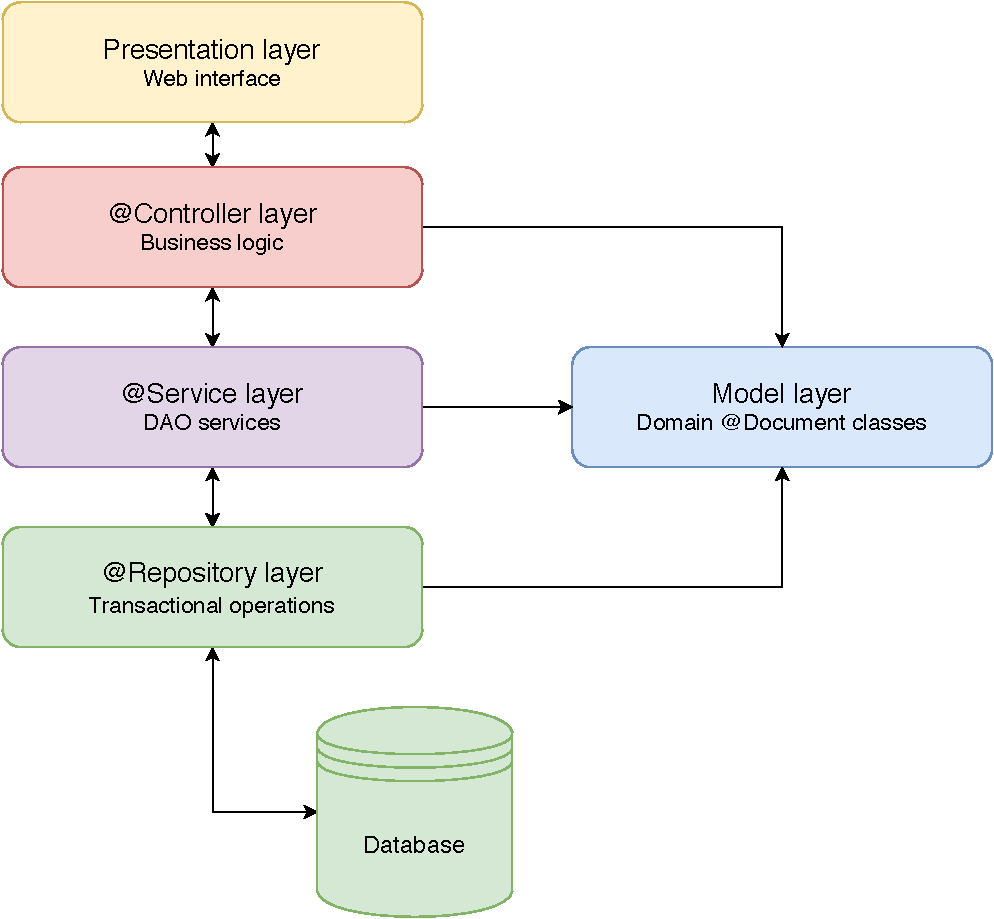
\includegraphics[width=0.8\linewidth]{4_layered-architecture}
	\caption[Layered architecture]{Layered architecture}
	\label{fig:layer_arch}
\end{figure}

\begin{figure}
	\centering
	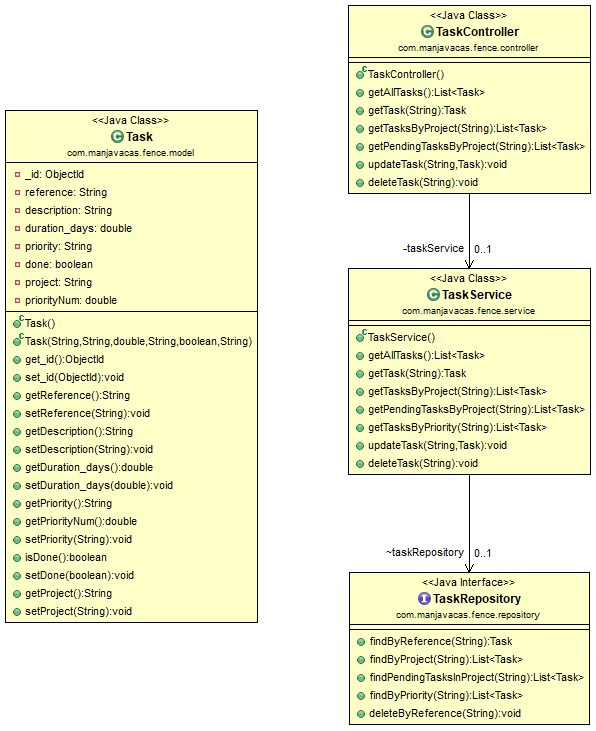
\includegraphics[width=0.65\linewidth]{4_sample-layers}
	\caption[Sample connection between layers]{Sample connection between layers}
	\label{fig:layers-sample}
\end{figure}

\begin{itemize}
\item \textbf{Presentation}. It is the layer in charge of the interaction with the user. In this case, it includes the static resources (HTML views and CSS code), as well as the underlying JavaScript code. This layer, conceived as the client side, communicates with the server through GET, POST, PUT or DELETE Ajax requests.
\item \textbf{Model}. This is the layer where the classes that model real-world entities are found. These classes, making use of the Spring framework integration with MongoDB, are labelled as documents (\textit{@Document}), so that they represent the basic structure of the documents included in the database's collections.
\item \textbf{Controller}. The controllers are the classes in charge of handling the CRUD requests received from the presentation layer. They make use of the classes defined in the Model layer, are labelled as \textit{@Controller}, and establish, for each of the CRUD operations, a mapping with their methods. In general, this layer covers business logic operations, so we can also find controller classes in charge of performing other transactions besides attending to requests from the presentation layer. Furthermore, when any of these operations requires access to the database, communication with the underlying DAO (Data Access Only) layers will be necessary.
\item \textbf{Service}. This layer includes the set of DAO classes that interact with the database. They are labelled as \textit{@Service} and include the logic needed to access repositories and handle controller requests.
\item \textbf{Repository}. Repository. MongoDB repositories are a type of interface included in Spring that provides easy and flexible interaction with MongoDB collections. They allow database queries to be abstracted and customized and are labelled as \textit{@Repository}. 
\end{itemize}

If we go deeper into the FENCE architecture at a class level, we will always find a similar pattern: the class controller attends to CRUD requests from the interface and, in case of requiring stored data, on request to the service class, the data is retrieved through the corresponding repository interface. This general procedure is summarized in Figure~\ref{fig:layer_int}.

\begin{figure}
	\centering
	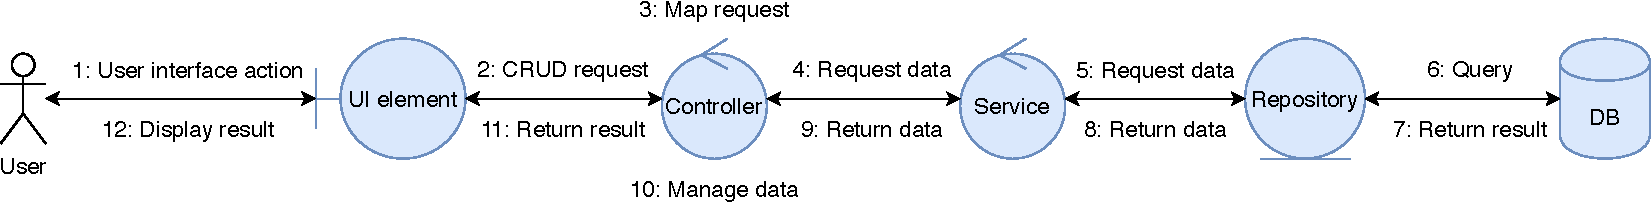
\includegraphics[width=0.95\linewidth]{4_layered-interaction}
	\caption[Layered interaction]{Layered interaction}
	\label{fig:layer_int}
\end{figure}

\subsubsection{DATA MODEL}

The reasons for using a noSQL database system like MongoDB are the advantages that this type of environments provide:

\begin{itemize}
\item On the one hand, they offer great flexibility during development, especially if we consider the easy integration of MongoDB with Spring framework.
\item On the other hand, the modification of noSQL schemes is very simple, fast, and scalable.
\item In addition, MongoDB databases also integrate SQL features and queries, so we can have the best of both types of databases in the same system.
\end{itemize}

However, although there are disadvantages when using noSQL, such as manual control of data consistency or operation atomicity, the data model of FENCE was not considered complex enough to make a SQL system more convenient.

As indicated, Spring's integration with MongoDB is relatively simple. We only need to label the classes we want to represent as database documents with \textit{@Document} in order to establish their schema. This will make it indexable through the \textit{@Repository} interfaces and easily accessible. An  of the correspondence between a class labelled as \textit{@Document} and its instance in the database is shown in Figure~\ref{fig:doc_sample}.

\begin{figure}
	\centering
	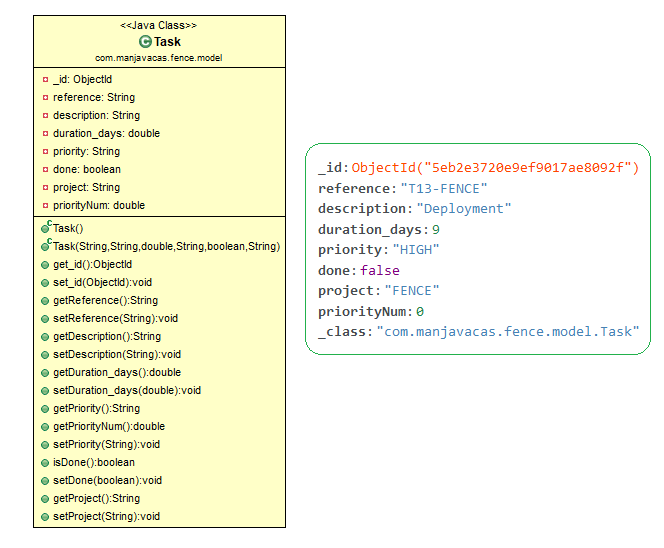
\includegraphics[width=0.65\linewidth]{4_sample-document}
	\caption[Relation between Java class and MongoDB document]{Relation between Java class and MongoDB document}
	\label{fig:doc_sample}
\end{figure}

On this basis, the scheme shown in Figure~\ref{fig:data_model} represents the data model of FENCE, where the \textit{@Document} classes and their relationships can be appreciated.

\begin{figure}
	\centering
	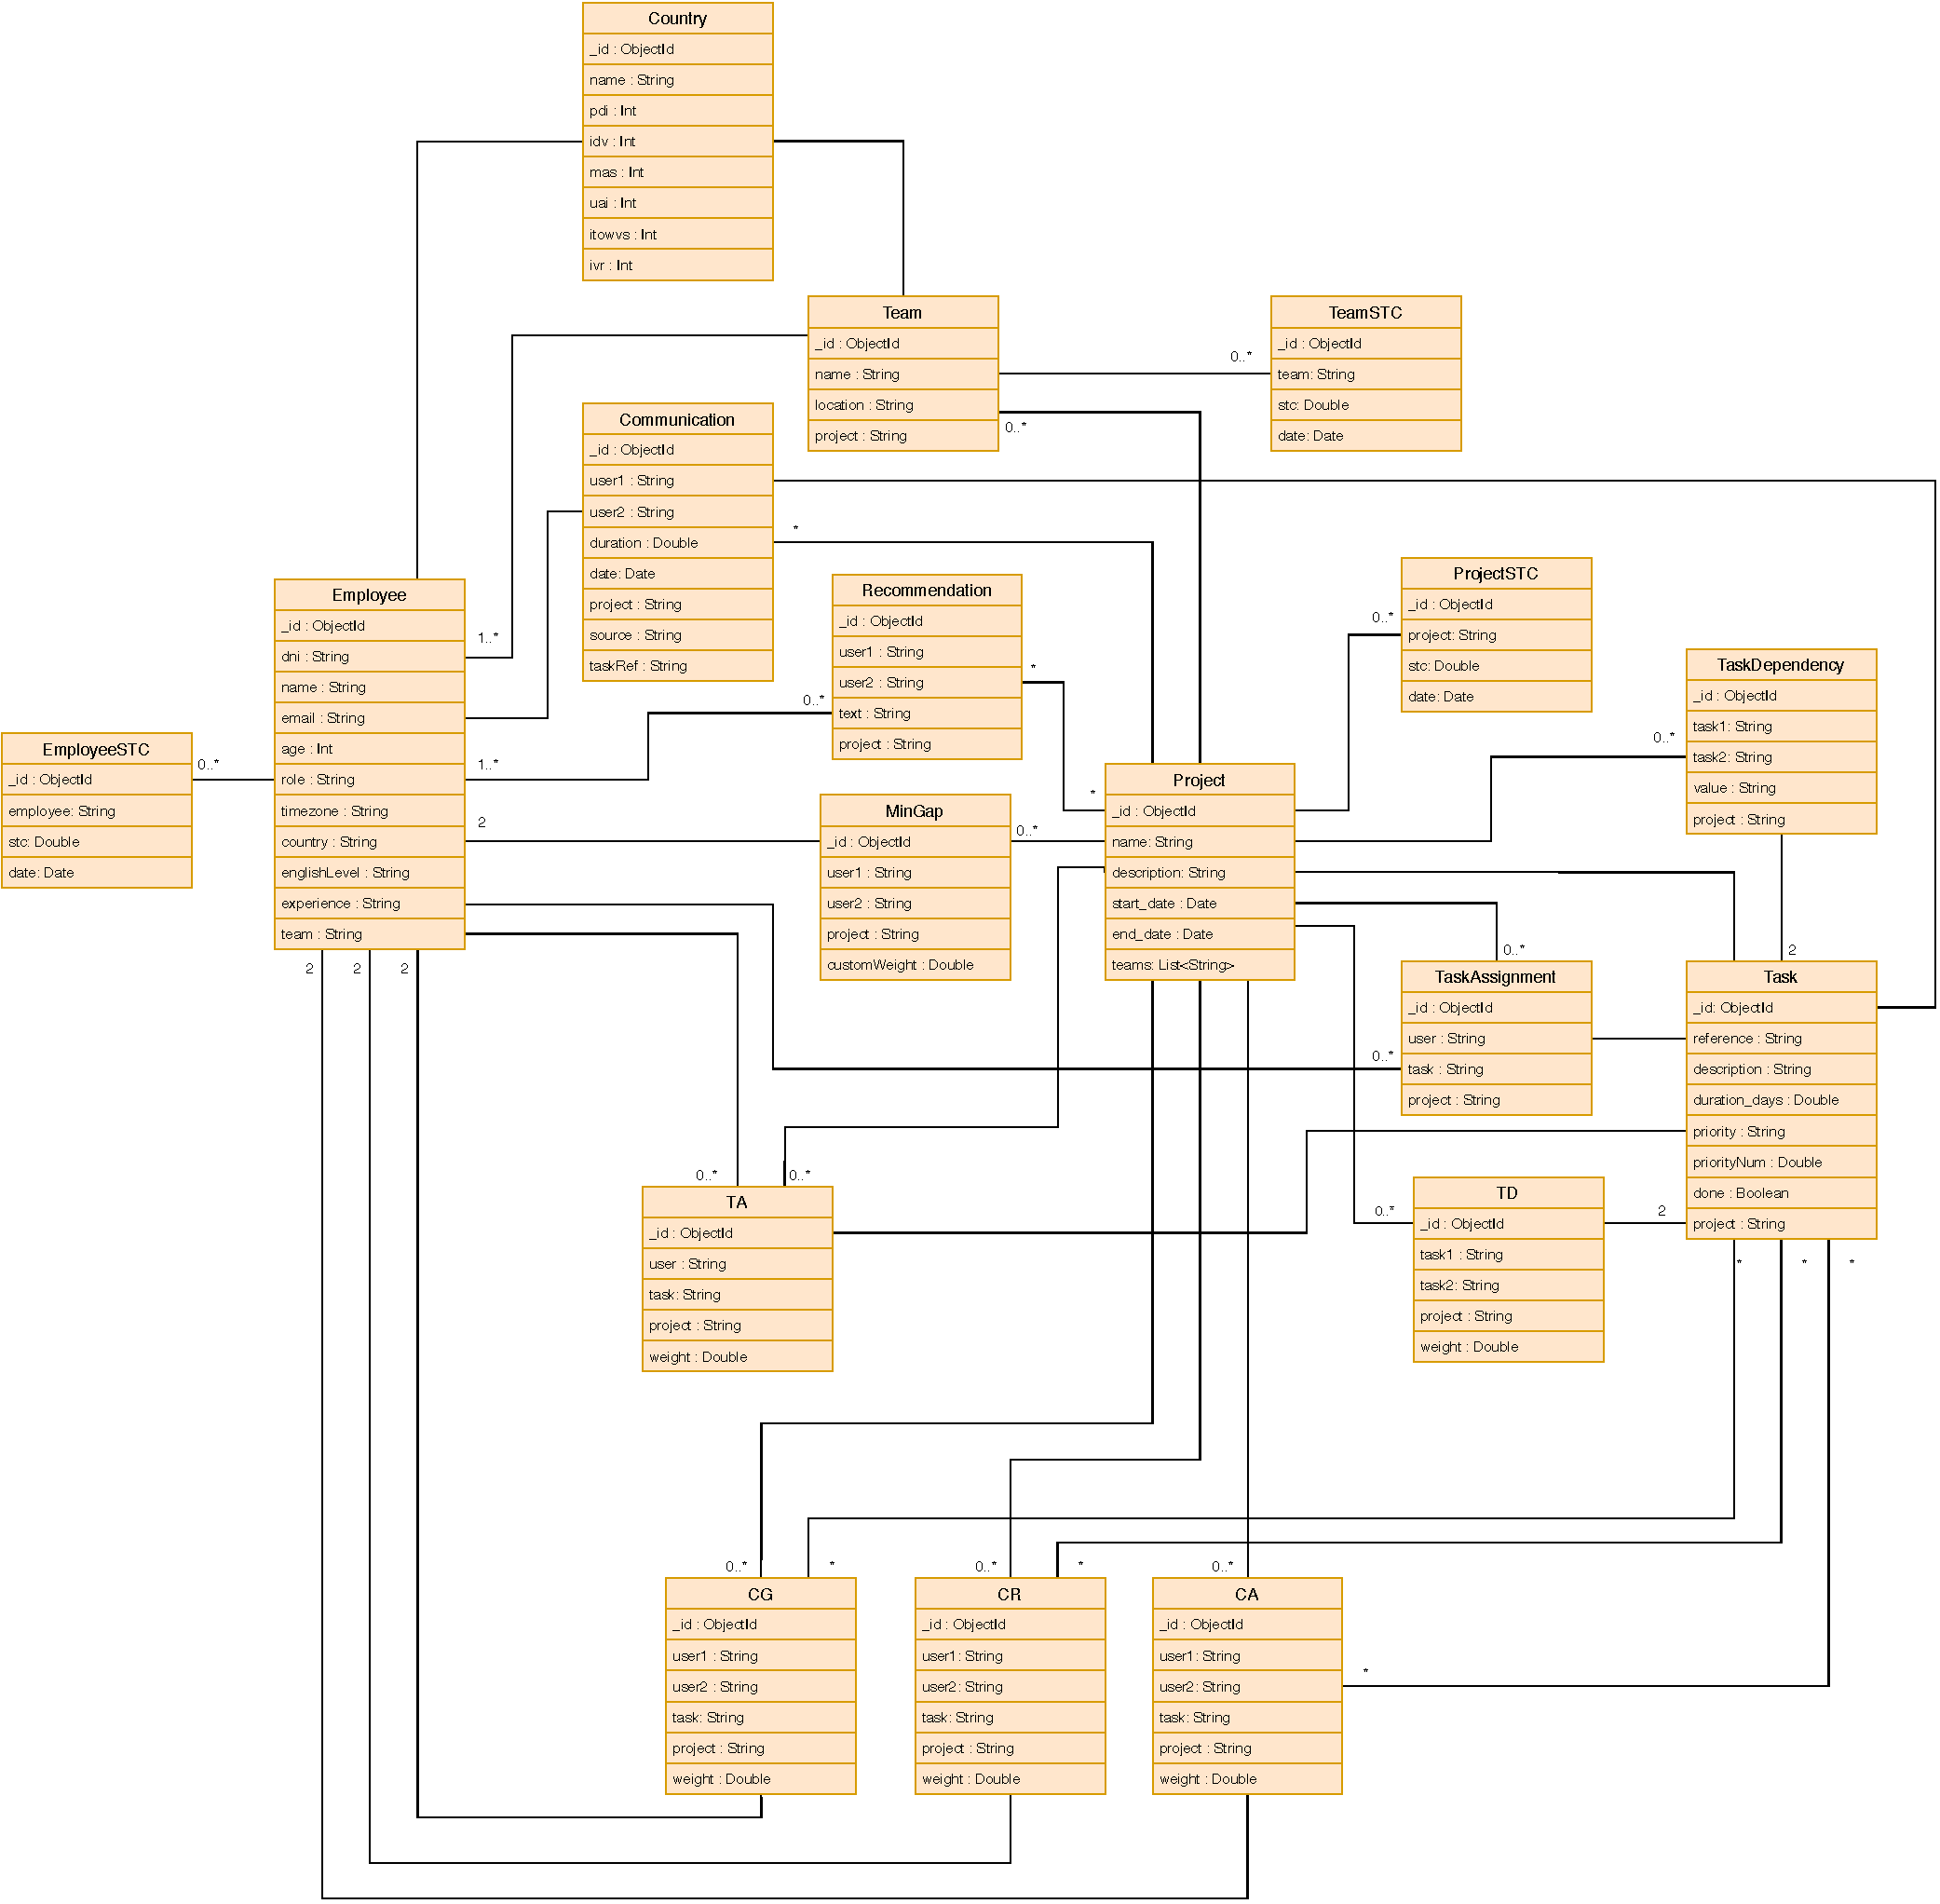
\includegraphics[width=0.95\linewidth]{4_data-model}
	\caption[FENCE data model]{FENCE data model}
	\label{fig:data_model}
\end{figure}

Therefore, once the architecture and data model of the system had been defined, the implementation of the different functional modules of FENCE was undertaken.

\section{Construction phase}

The following subsections will address in detail the process of developing the functionalities of FENCE, as well as the difficulties and decisions faced in its implementation. The implementation of each of these modules meant a micro-increment in the functionalities of FENCE, giving as a result the first version of the application.

\subsection{Module 1. API skeleton}

The first objective pursued in this phase was the creation of the initial set of resources that compose the application, as well as the main windows that would define the structure of the system's interface. Throughout this stage, the main structure of the data model was established, which would be progressively expanded throughout the project.

Thus, taking as a reference this initial data model and the previously designed class diagram, the different classes, URIs and query methods were defined. Likewise, as shown in Figure~\ref{fig:mongodb-cluster}, the MongoDB cluster hosted in the MongoDB Atlas cloud service was created, establishing access permissions, integrating the MongoDB Java Driver into the Maven project, and making queries operational through Spring.

\begin{figure}
	\centering
	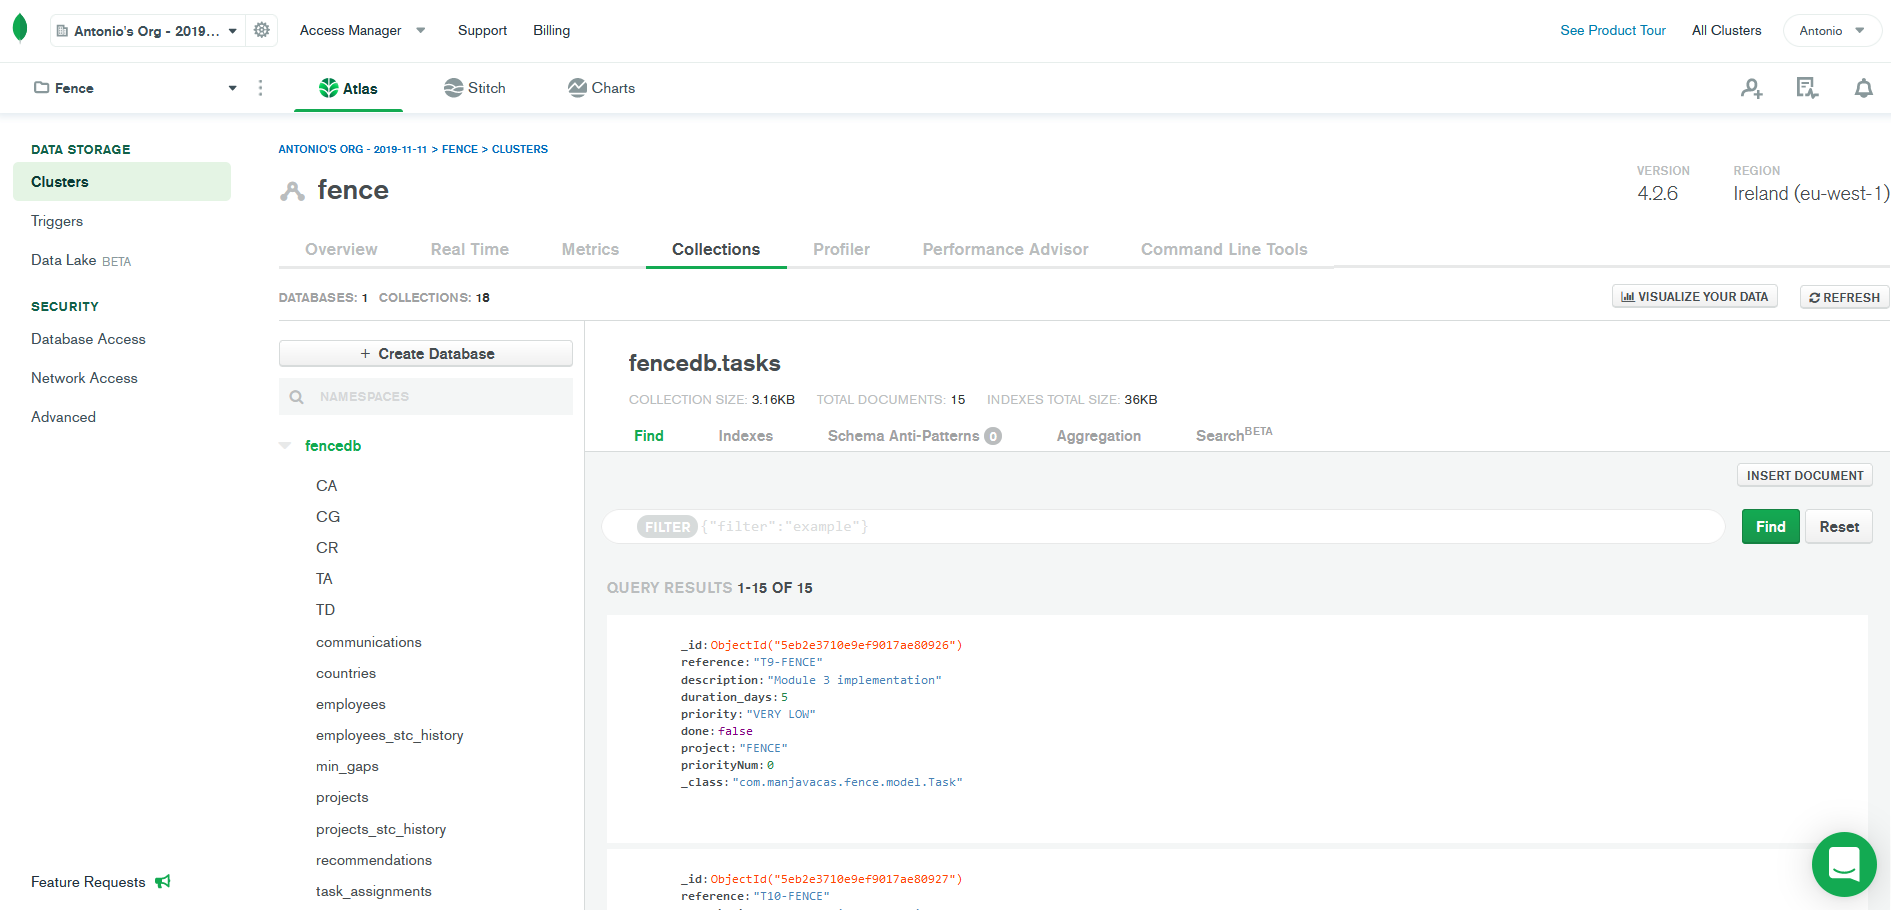
\includegraphics[width=0.95\linewidth]{4_mongodb-atlas}
	\caption[MongoDB Atlas cluster]{MongoDB Atlas cluster}
	\label{fig:mongodb-cluster}
\end{figure}

Once the cluster’s database was created and correctly integrated into the system, the main CRUD operations were added for each of the resources, defining the necessary methods in Controllers, Services and Repositories. Following the model provided by Spring framework, each application resource is represented by a class from the Model package, as previously explained. On the other hand, controllers are in charge of the main operations and communication with the interface, while service classes act as DAO entities communicating with the MongoDB repositories (as shown in Figure~\ref{fig:layer_arch}).

Therefore, when the logical skeleton of the application had been created, the two main windows of the system were elaborated. On the one hand, the main control panel that would be gradually completed in the different iterations of the project, whose first version is shown in Figure~\ref{fig:first-dashboard}.

\begin{figure}
	\centering
	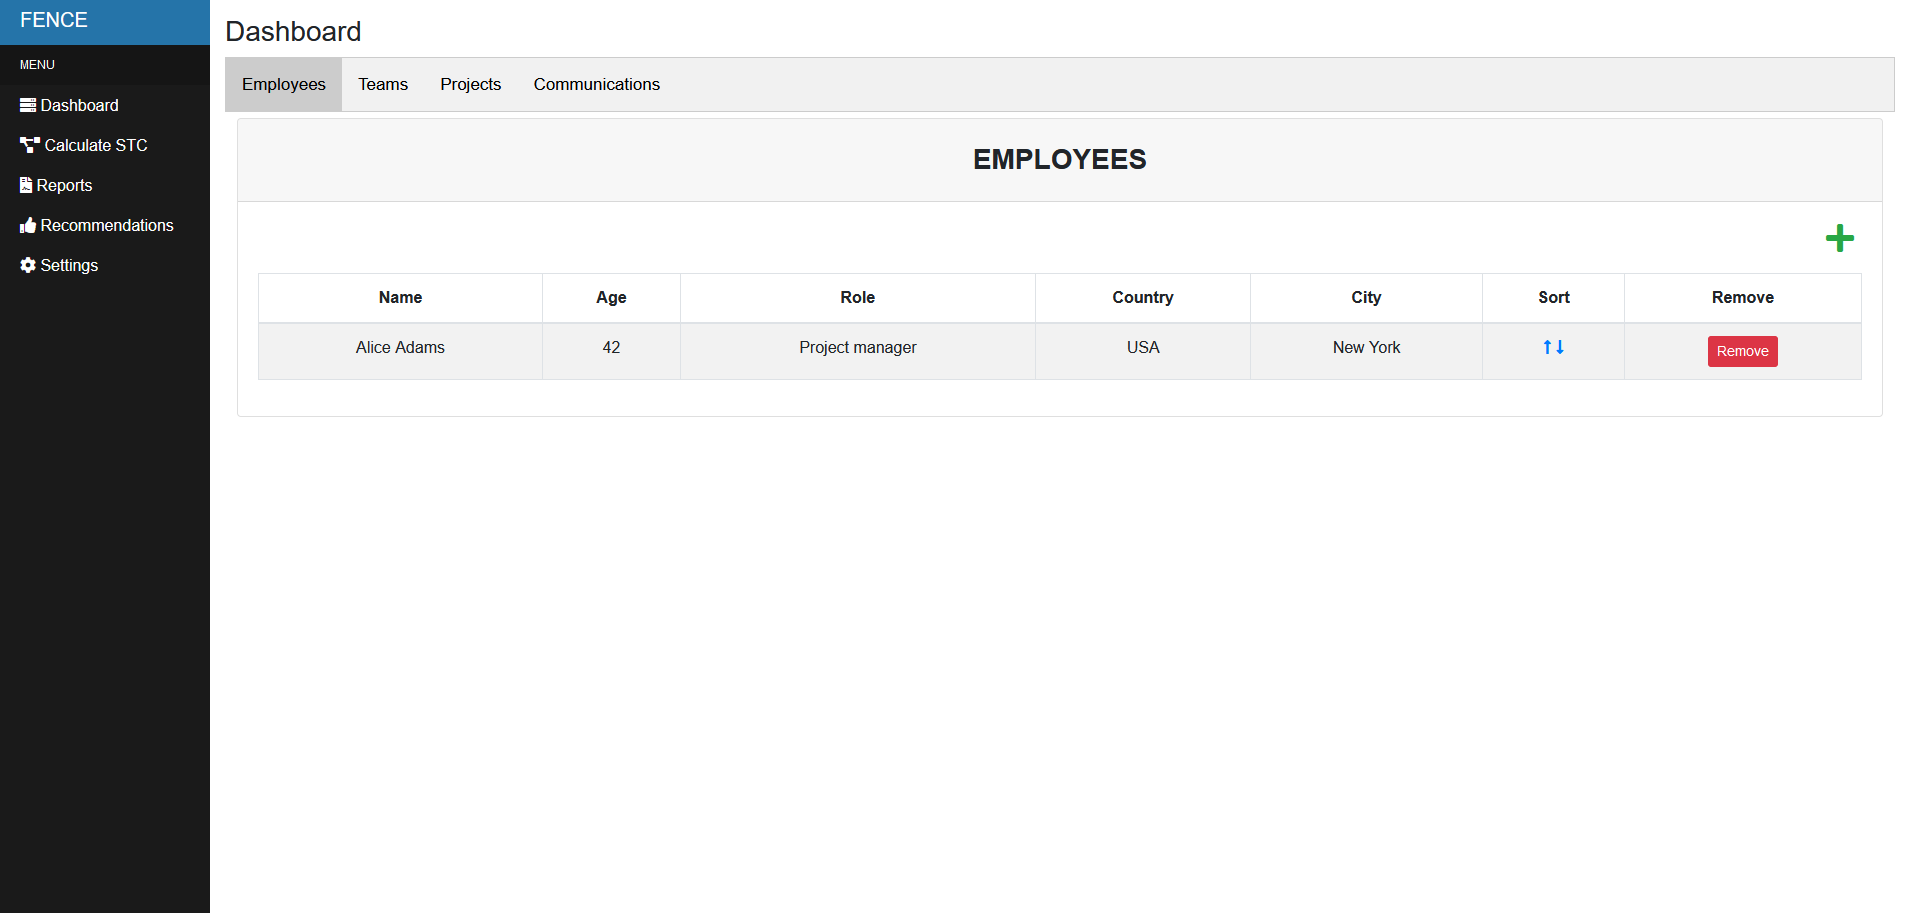
\includegraphics[width=0.95\linewidth]{4_first-dashboard}
	\caption[First dashboard version]{First dashboard version}
	\label{fig:first-dashboard}
\end{figure}

On the other hand, a home page was developed with information about the utility, version, and authorship of FENCE, whose final version is shown in Figure~\ref{fig:home-page}.

\begin{figure}
	\centering
	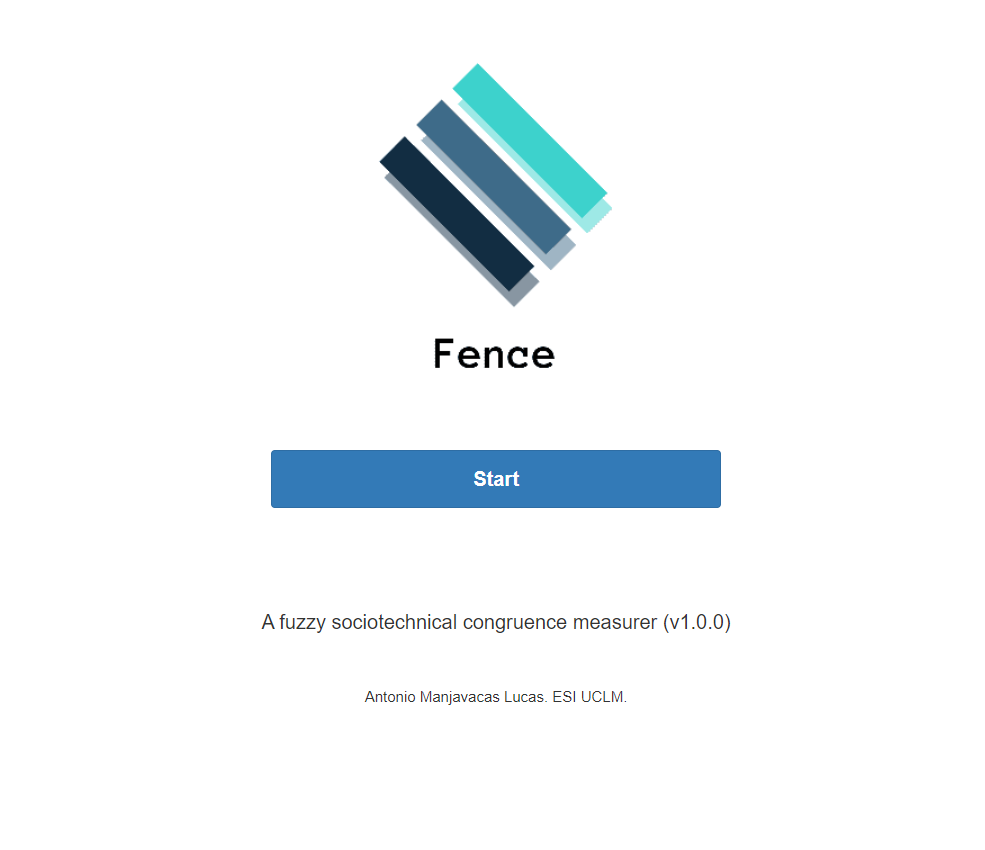
\includegraphics[width=0.8\linewidth]{4_home-page}
	\caption[FENCE home page]{FENCE home page}
	\label{fig:home-page}
\end{figure}

\subsection{Module 2. Main user interface}

In this second construction stage, efforts were focused on improving and completing the interface outlined in the previous module. This implied a greater deepening in HTML, CSS and JavaScript solutions, making use of Bootstrap and jQuery as nexus to implement the different functionalities of the interface. Initially, the use of these technologies never employed was an individual challenge, and therefore much of the effort invested at this stage was related with learning them.

An objective pursued in this stage was the elaboration of the different tabs and panels that compose the system's dashboard, as well as the communication between the interface and the application controllers via jQuery's Ajax requests. These requests were carried out according to the controllers' URIs defined in the previous construction stage, following the communication model expressed in Figure~\ref{fig:layer_int}.

\begin{figure}
	\centering
	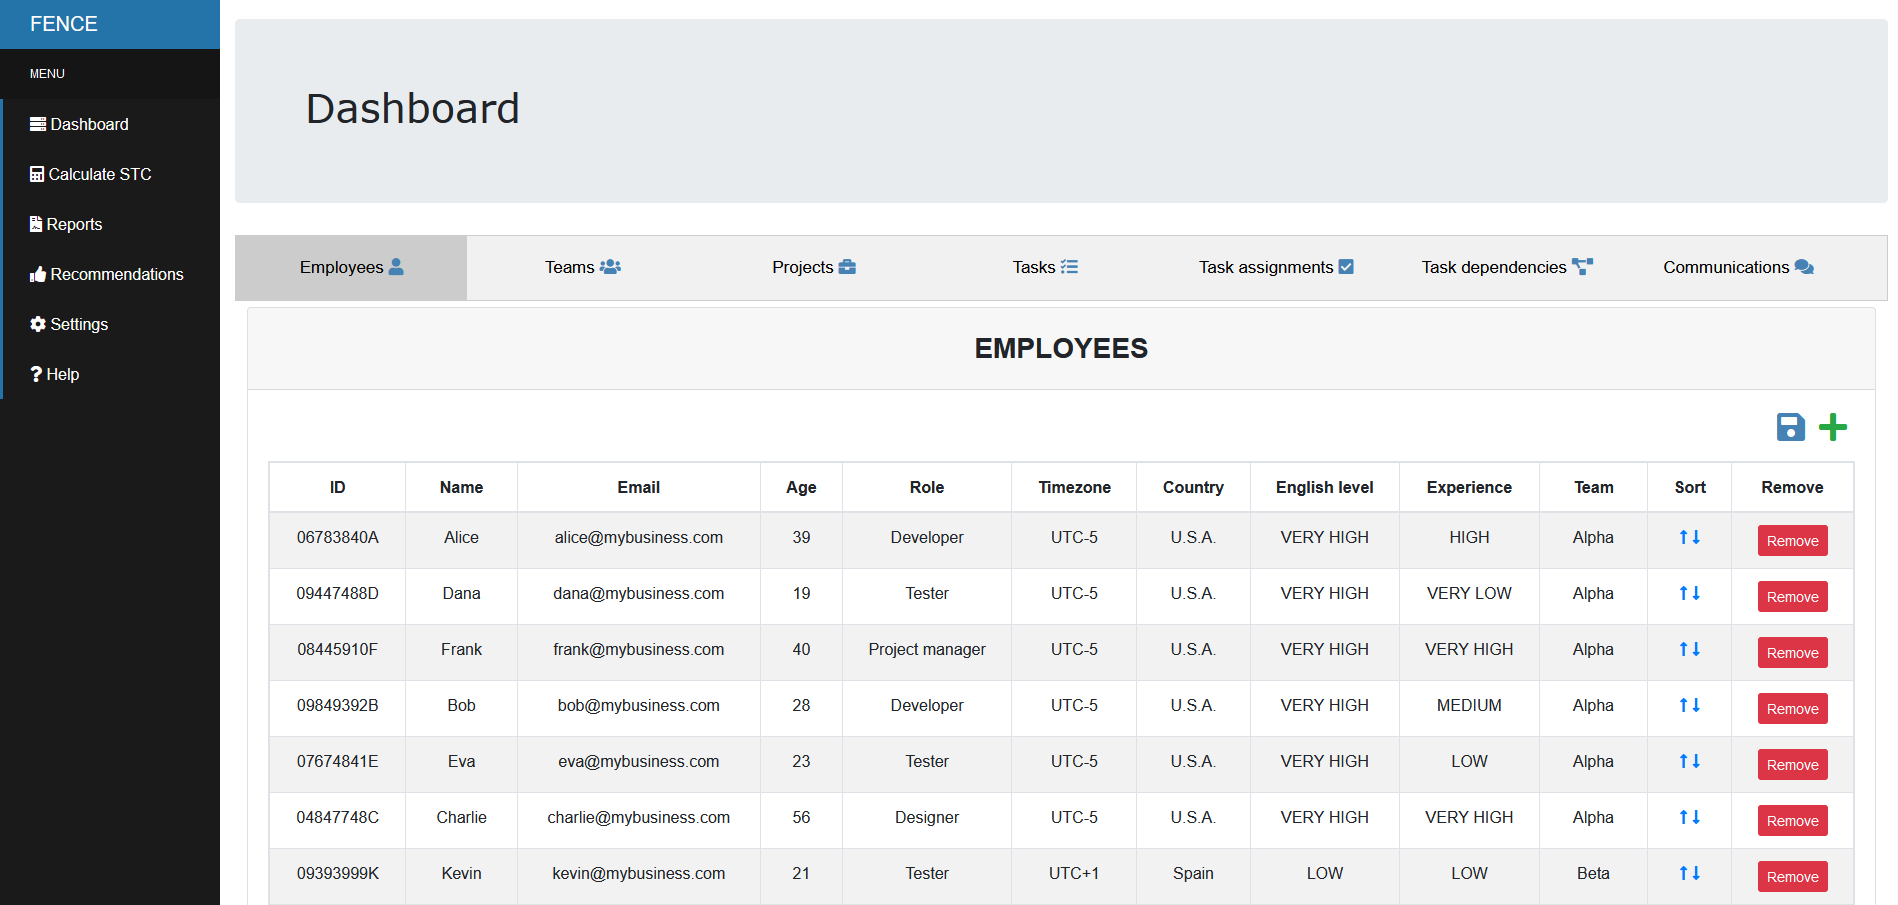
\includegraphics[width=0.95\linewidth]{4_fence-dashboard}
	\caption[FENCE dashboard]{FENCE dashboard}
	\label{fig:fence-dashboard}
\end{figure}

Furthermore, as can be seen in the Figure~\ref{fig:fence-dashboard}, these were the tabs contained the dashboard in its final version:

\begin{itemize}
	\item \textbf{Employees}: includes information on the users that are part of the organisation, used to measure individuals’ STC, such as age, experience, English level, country, etc.
	\item \textbf{Teams}: includes the name, location, and project membership of the different teams in the organization.
	\item \textbf{Projects}: active projects in the organization.
	\item \textbf{Tasks}: tasks to be carried out in each of the projects, together with their description, duration, priority, and completion.
	\item \textbf{Task assignments}: information about task assignment to users.
	\item \textbf{Task dependencies}: information on dependencies between tasks and their reliance weight.
	\item \textbf{Communications}: communications history between users. We will see in future sections their utility and how they are gathered.
\end{itemize}

Once the dashboard was implemented and the main application windows were set, some test data was loaded, while the proper performance of methods and queries were tested.

\subsection{Module 3. STC measurement}
\label{sec:stc}

Up to now, the creation of the main resources of the tool, their storage, and the CRUD interaction with them through the dashboard have been presented. In this stage, the objective pursued was to use these resources to carry out the measurement of the STC at the different levels of the organization under consideration: users, teams, and projects.

As previously explained in chapter \ref{cap:introduction}, the procedure taken as a reference to measure STC was the one exposed by Kwan et al. \cite{kwan_weighted_2009,kwan_does_2011}, given its facility to be adapted to the features and requirements of FENCE. Therefore, in the following subsections we will see gradually how the STC is calculated through the different algorithms implemented in this module:

\subsubsection{TASK ASSIGNMENT MATRIX ($T_A$)}

The first step in computing STC levels is to construct the task assignment matrix ($T_A$). This matrix matches tasks with users, representing the degree of user involvement in the tasks assigned to them (see Figure~\ref{fig:ta-matrix}).

\begin{figure}
	\centering
	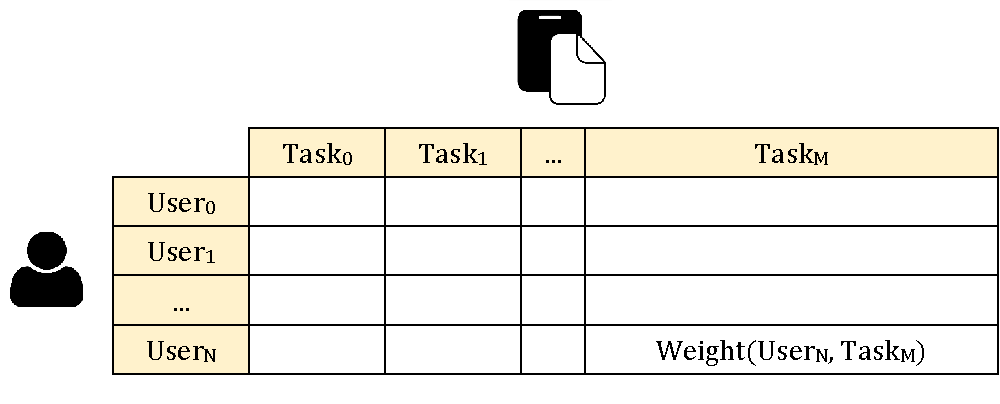
\includegraphics[width=0.95\linewidth]{4_ta-matrix}
	\caption[$T_A$ matrix]{$T_A$ matrix}
	\label{fig:ta-matrix}
\end{figure}

Both for this case and for the rest of the matrices detailed in the literature, in order to reduce the complexity and computational cost of the algorithms, these matrices were replaced by lists of objects stored in the database. In this case, the class $T_A$ represents a concrete cell in the $T_A$ matrix, as shown in Figure~\ref{fig:ta-class}. Moreover, the process carried out to fill in this matrix consists on the one shown in Algorithm~\ref{alg:ta}.

\begin{figure}
	\centering
	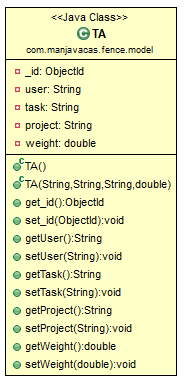
\includegraphics[width=0.32\linewidth]{4_ta-class}
	\caption[$T_A$ class]{$T_A$ class}
	\label{fig:ta-class}
\end{figure}

\begin{algorithm}
    
    \DontPrintSemicolon
    \SetKwInOut{Input}{input}
    \SetKwInOut{Output}{output}
    \Input{project}
    \Output{$T_A$ matrix}
    
    \caption{$T_A$ calculation}
    \label{alg:ta}
        
        $taMatrix \longleftarrow $\O$ $\;
        $tasks \longleftarrow getPendingTasks(project) $\;
        
        \ForEach{$task$ in $tasks$}{
            $users \longleftarrow getUsersAssignedTo(task) $\;
            
            \If{users $\ne$ \O}{
                $sumExp \longleftarrow sumExperiences(users) $\;
                
                \ForEach{user $td$ in $users$}{
                    $weight \longleftarrow (user.experience / sumExp) * task.priority $\;
                    
                    \If{weight $>$ 1}{weight $\longleftarrow$ 1}
                    
                    $taMatrix \cup T_A(user, task, weight, project)$\;
                }
            }
        }
    
\end{algorithm}

Finally, the generated records are stored in the database replacing older ones, always keeping the most up-to-date $T_A$ matrix in the database.

\subsubsection{TASK DEPENDENCY MATRIX ($T_D$)}

The task dependency matrix ($T_D$) is very similar to the previous one, except that in this case the matrix does not relate users to tasks but tasks to each other. Specifically, what this matrix reflects is the degree of dependency between tasks in a project (see Figure~\ref{fig:td-matrix}). As this dependency level is flexible, it can be adapted to the user's understanding of "dependency". For example, the weight of the dependency between two tasks may reflect the number of functionalities of one task that must be previously implemented to perform the other.

\begin{figure}
	\centering
	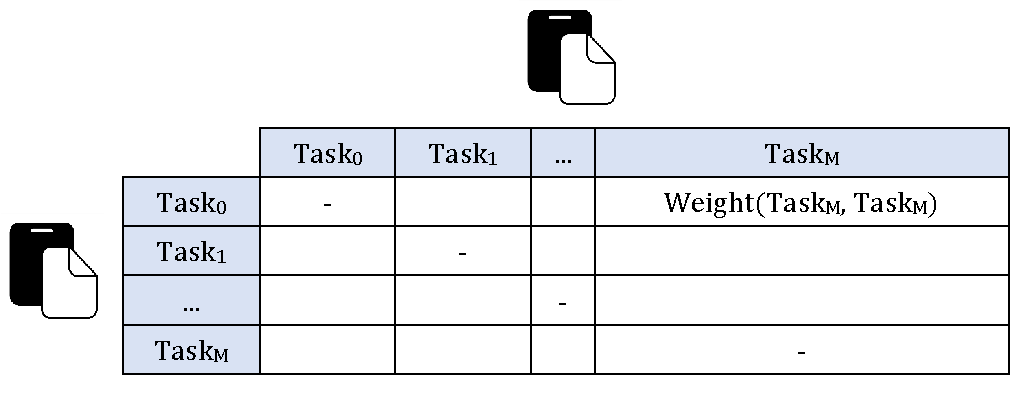
\includegraphics[width=0.95\linewidth]{4_td-matrix}
	\caption[$T_D$ matrix]{$T_D$ matrix}
	\label{fig:td-matrix}
\end{figure}

As in the previous case, the different cells of the $T_D$ matrix are stored as objects in the database (see Figure~\ref{fig:td-class}). The process of their creation is the one shown in Algorithm~\ref{alg:td}.

\begin{figure}
	\centering
	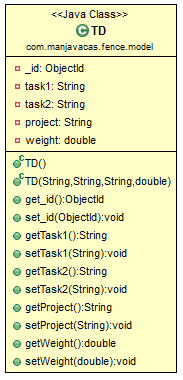
\includegraphics[width=0.32\linewidth]{4_td-class}
	\caption[$T_D$ class]{$T_D$ class}
	\label{fig:td-class}
\end{figure}

\begin{algorithm}
    
    \DontPrintSemicolon
    \SetKwInOut{Input}{input}
    \SetKwInOut{Output}{output}
    \Input{project}
    \Output{$T_D$ matrix}
    
    \caption{$T_D$ calculation}
    \label{alg:td}
        
        $tdMatrix \longleftarrow $\O$ $\;
        $tasks \longleftarrow getPendingTasksOf(project) $\;
        
        \ForEach{$task$ in $tasks$}{
            $taskDependencies \longleftarrow getDependenciesOf(task) $\;
            
            \If{taskDependencies $\ne$ \O}{
                $sumValues \longleftarrow sumWeights(taskDependencies) $\;
                
                \ForEach{taskDependency in $taskDependencies$}{
                    $weight \longleftarrow taskDependency.weight / sumValues $\;
                    $tdMatrix \cup T_D(task, taskDependency, weight, project)$\;
                }
            }
        }
    
\end{algorithm}

Both the calculation of $T_D$ and $T_A$ is relatively quick, since the operations performed consist mainly on entering the information provided by the user in objects that are stored in the database. However, this is not the case of the $C_R$ and $C_A$ matrices, which will be presented in the following subsections.

\subsubsection{COMMUNICATION REQUIREMENTS MATRIX ($C_R$)}

Once the $T_A$ and $T_D$ matrices are obtained, we can compute the coordination requirements between users represented in the $C_R$ matrix (see Figure~\ref{fig:cr-matrix} and Figure~\ref{fig:cr-class}). This matrix represents the communication needs between user pairs based on the tasks assigned to them and their dependencies. In this case, the weights of the different matrix cells represent how much the users involved must coordinate.

\begin{figure}
	\centering
	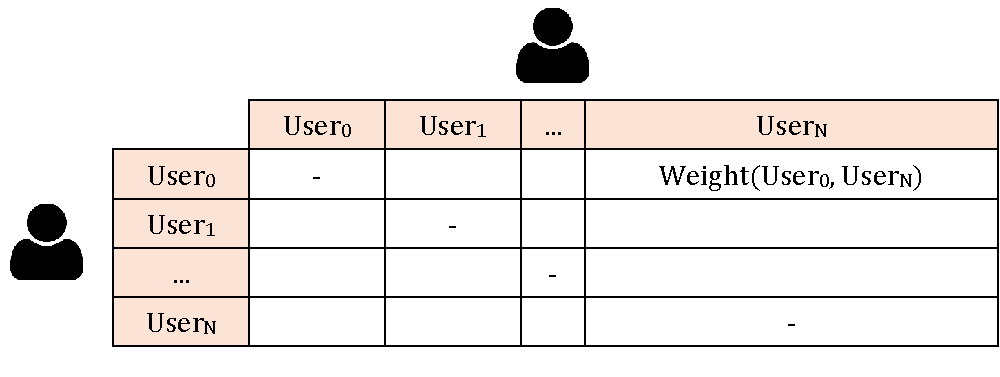
\includegraphics[width=0.95\linewidth]{4_cr-matrix}
	\caption[$C_R$ matrix]{$C_R$ matrix}
	\label{fig:cr-matrix}
\end{figure}

\begin{figure}
	\centering
	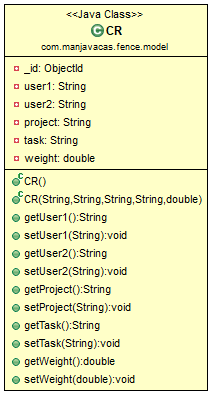
\includegraphics[width=0.32\linewidth]{4_cr-class}
	\caption[$C_R$ class]{$C_R$ class}
	\label{fig:cr-class}
\end{figure}

Initially calculated by means of the operations shown in Equation~\ref{eq:cr}, in this case we will follow an iterative procedure to calculate these coordination requirements, as no matrices are being used:

\begin{equation}
	\label{eq:cr}
	C_R = T_A * T_D * T_A^T
\end{equation}

As can be shown in Algorithm~\ref{alg:cr}, in the calculation of the weights for each coordination requirement, this weight is subsequently adjusted according to different distances present in Global Software Development projects. Thus, a fuzzy inference system is used to carry out this adjustment, whose objective is none other than trying to reflect the difficulties or "penalties" to communication that may be caused by socio-cultural, geographical, or temporal distances among users.

\begin{algorithm}
    
    \DontPrintSemicolon
    \SetKwInOut{Input}{input}
    \SetKwInOut{Output}{output}
    \Input{project, $T_A$ matrix, $T_D$ matrix}
    \Output{$C_R$}
    
    \caption{$C_R$ calculation}
    \label{alg:cr}
        
        $crMatrix \longleftarrow $\O$ $\;
        
        \ForEach{taskAssignment $ta$ in $taMatrix$}{
           
           $user_1 \longleftarrow ta.user $\;
           $dependencies \longleftarrow getDependenciesOf(ta.task) $\;
           
            \ForEach{taskDependency $td$ in dependencies}{
             
                $responsibles \longleftarrow getUsersAssignedTo(td.task_2)$\;
               
               \ForEach{user $user_2$ in responsibles} {
                    
                    \If{$user_2$ $\ne$ $user1$} {
                        $weight_{T_A}1 \longleftarrow ta.weight$ \;
                        $weight_{T_A}2 \longleftarrow T_A(td.task_2, user_2).weight$ \;
                        $weight_{T_D} \longleftarrow T_D(ta.task, td.task_2).weight$ \;
                        \;
                        $weight \longleftarrow weight_{T_A}1 * weight_{T_A}2 * weight_{T_D}$ \;
                        $weight \mathrel{{+}{=}} computeGlobalFactors(user_1, user_2)$ \;
                        \;
                        \If{weight $>$ 1}{weight $\longleftarrow$ 1}\;
                        $crMatrix \cup C_R(user_1, user_2, ta.task, weight, project)$\;
                    }
               }
               
            }
        }
    
\end{algorithm}

The entries taken by the fuzzy inference system are the following:

\begin{itemize}
\item \textbf{Common English level}. Level of English shared by users, assuming that communication between them is always in this language despite their country provenance. It can be assumed that even if two users communicate in their native language, the level of English must be considered if the information disseminated by public chats (i.e. Jira, GitHub, Teams, Slack, etc.) should be interpretable by other users. Depending on the individual level of each user, the following weights are assessed:\newline

	\begin{itemize}
	\item If both users have a high level of English, the common level of English is 1.
	\item If one user has a high level and the other has a medium level, the weight is 0.7.
	\item If both have a medium level of English, the common level of English is 0.5.
	\item On the other hand, if one user has a medium level of English and the other has a low level, the resulting weight is 0.3.
	\item Finally, if both users have a low level of English the common weight is 0.\newline
	\end{itemize} 
	
	Moreover, the fuzzy sets associated with this variable are shown in the Figure~\ref{fig:fs-english}.\newline
	
	\begin{figure}
		\centering
		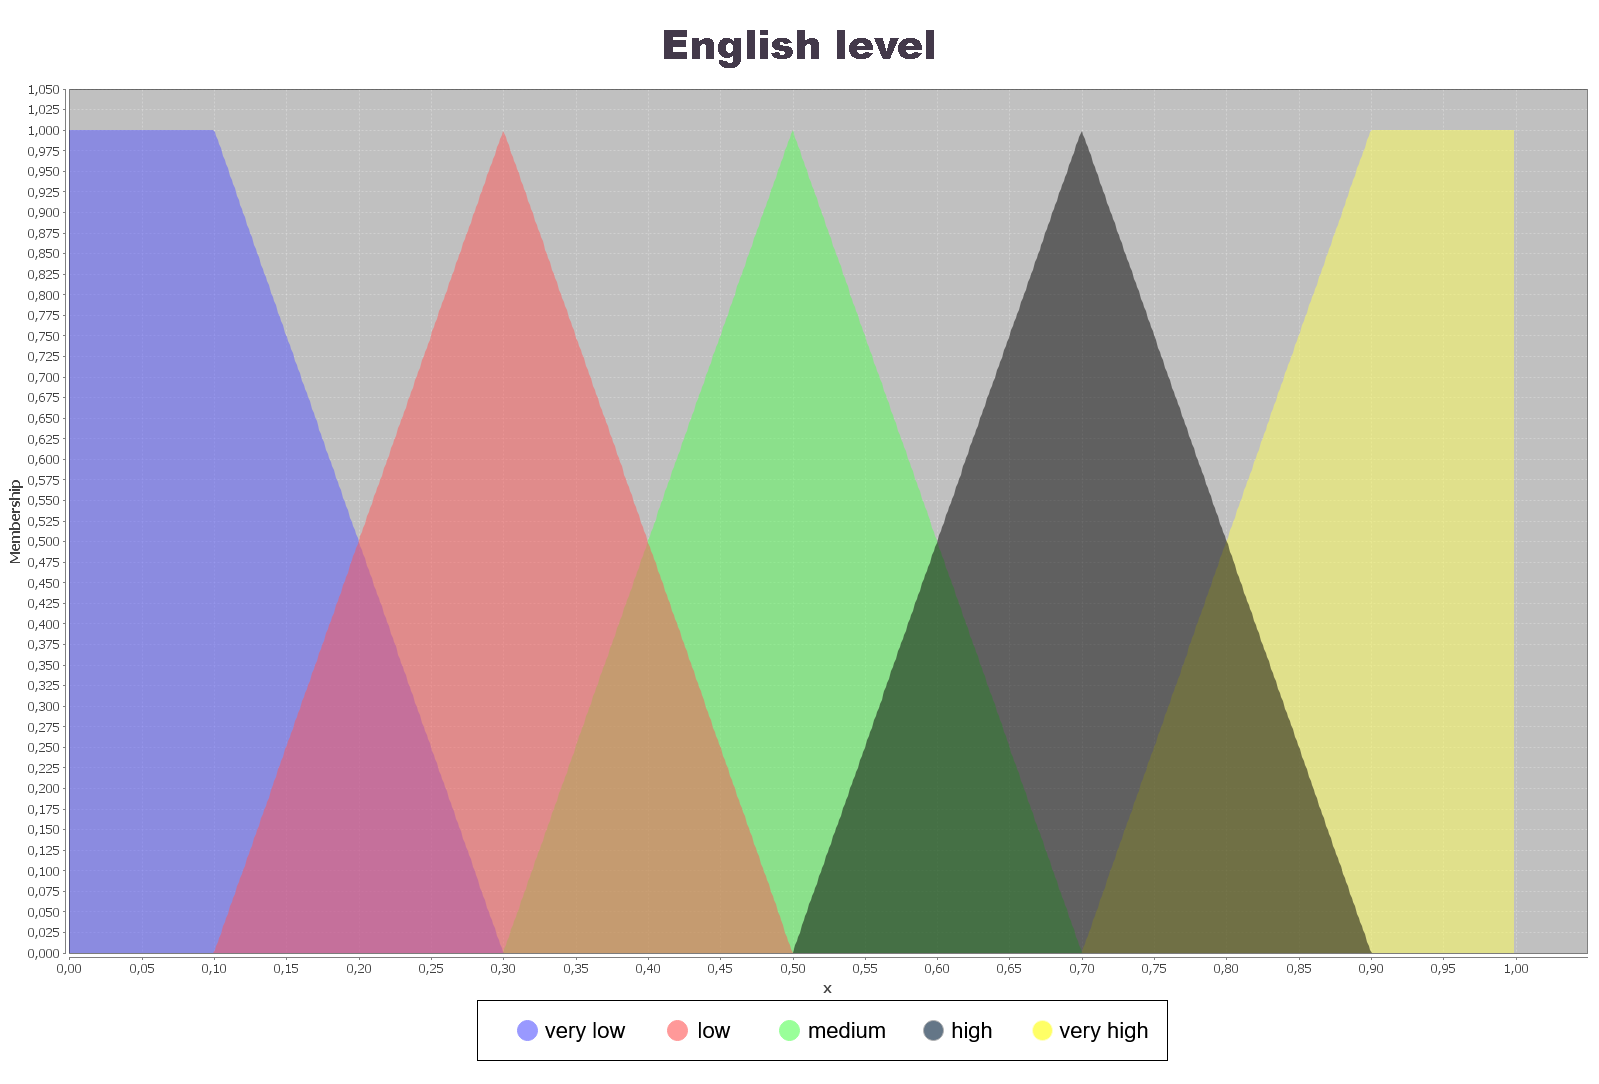
\includegraphics[width=0.9\linewidth]{4_fuzzy-sets-english}
		\caption[English level fuzzy sets]{English level fuzzy sets}
		\label{fig:fs-english}
	\end{figure}

\item \textbf{Cultural distance}. Average of the distances between socio-cultural factors identified by G. Hofstede \cite{hofstede_cultures_2004}, according to the employees’ nationality\footnote{These socio-cultural factors have been quantified by experts and are freely available for academic research purposes at \url{https://geerthofstede.com/research-and-vsm/dimension-data-matrix/}.}. These are the ones deeply explained in \cite{hofstede_dimensions}, \cite{hofstede_compare}:\newline

	\begin{itemize}
	\item \textbf{Power distance} (PDI): degree of acceptance of power differences or equality in society. In societies with higher PDI, higher social classes are more questioned, while in cultures with lower PDI, there is more equal power among people.
	\item \textbf{Individualism} (IDV): defines the level of integration of individuals into society and the development of a sense of group membership. Compared to more individualistic countries we find others with a collectivist orientation.
	\item \textbf{Masculinity} (MAS): defines a culture's tendency towards more masculine or feminine patterns of behaviour. According to Hofstede, male societies are more assertive, competitive and focused on outcomes than the generally more empathetic female societies.
	\item \textbf{Uncertainty avoidance} (UAI): acceptance of situations of uncertainty or where there is no absolute truth. It represents the degree of relativism of societies.
	\item \textbf{Long term orientation} (LTO): this cultural factor differentiates between more traditionalist societies, with long-term aspirations, and those with short-term orientations where social relations are seen as a means to gain some kind of benefit.
	\item \textbf{Indulgence} (IVR): explains the vision of life that every culture has. On the one hand, indulgent cultures tend to be more optimistic and positive than contained cultures. On the other hand, contained cultures consider a more reserved enjoyment.\newline
	\end{itemize}

	Thus, all these factors were inserted in a collection where each document represents a country with the cultural features differentiated in the mentioned study.\newline
	
	On this basis, the cultural distance (CD) is calculated by following the Equation~\ref{eq:cult-dist}.
	
	\begin{equation}
		\label{eq:cult-dist}
		CD = \frac{\left| pdi_1 - pdi_2 \right| + \left| idv_1 - idv_2 \right| + \left| mas_1 - mas_2 \right| + \left| uai_1 - uai_2 \right| + \left| lto_1 - lto_2 \right| + \left| ivr_1 - ivr_2 \right|}{6}
	\end{equation}
	
	Similarly, the fuzzy sets considered for this variable are shown in the Figure~\ref{fig:fs-cultural}.\newline

	\begin{figure}
		\centering
		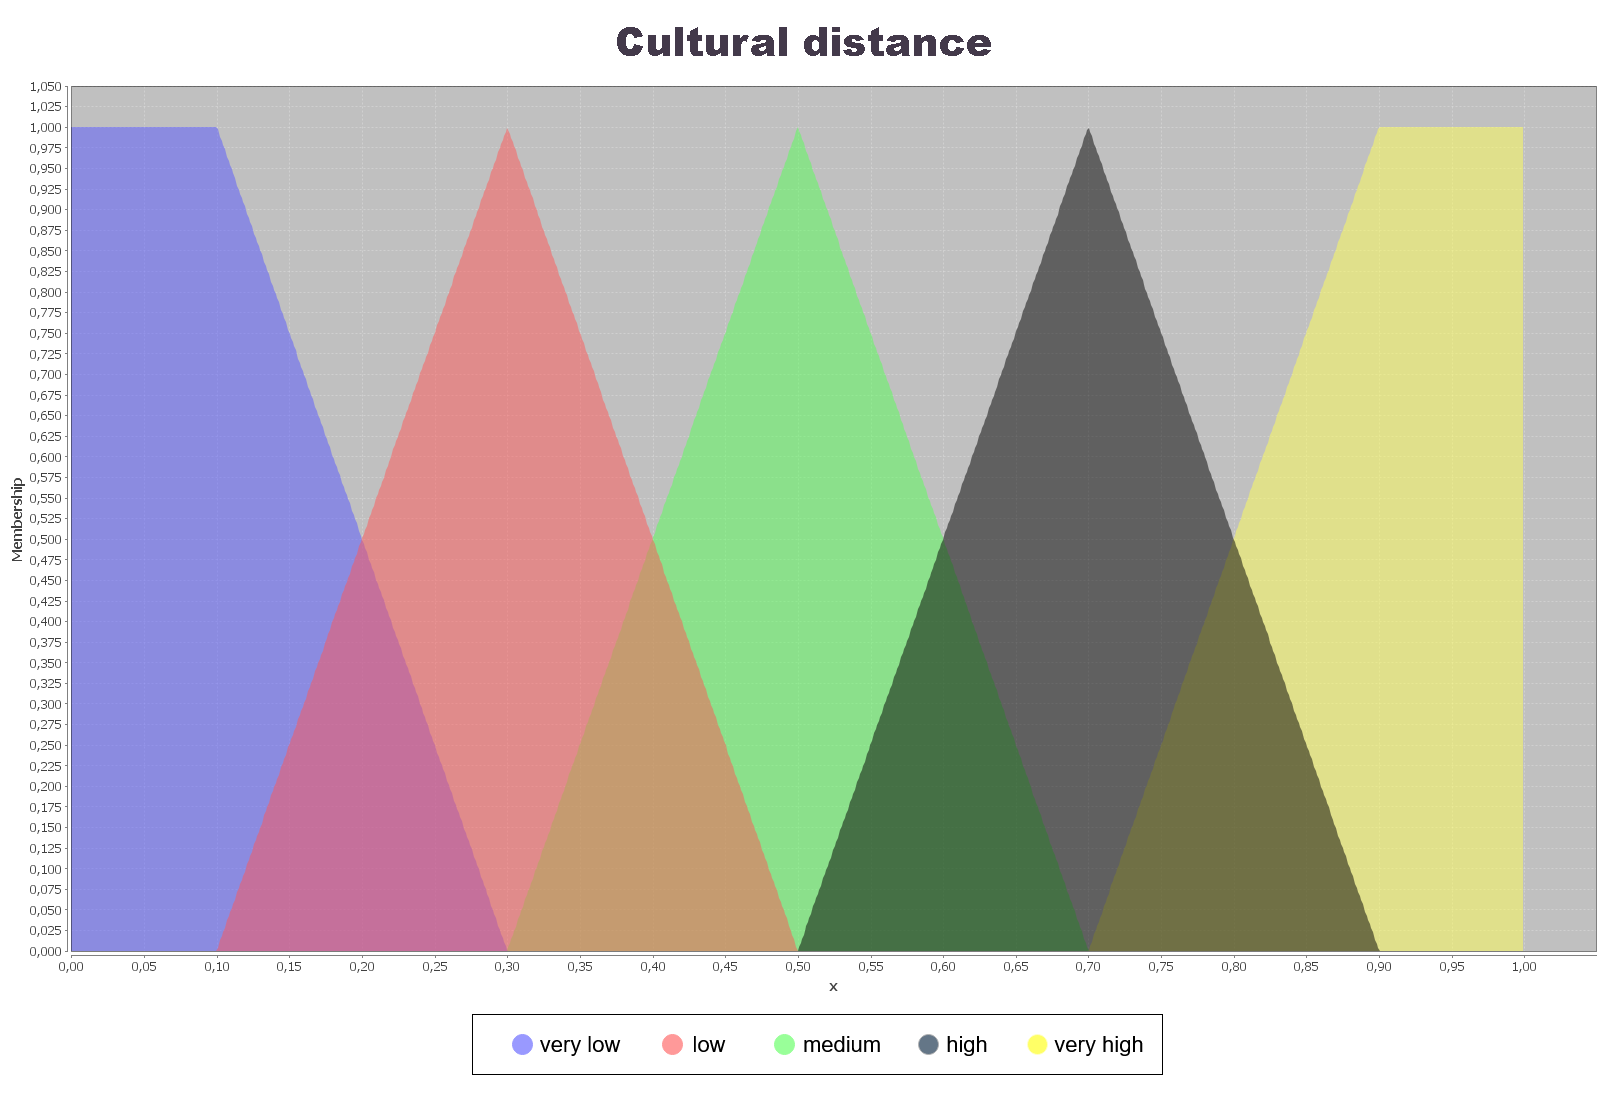
\includegraphics[width=0.9\linewidth]{4_fuzzy-sets-cultural}
		\caption[Cultural distance fuzzy sets]{Cultural distance fuzzy sets}
		\label{fig:fs-cultural}
	\end{figure}
	
\item \textbf{Time overlap}. Coincidence between employees’ time zones (UTC), calculated as the inverse of their time difference. A greater time overlap will facilitate the use of synchronous means of communication, while the impossibility of temporal coincidence in communication will result in greater use of asynchronous means. The computation of the time overlap is carried out following the Equation~\ref{eq:time-diff}, while the considered fuzzy sets for this input variable are shown in the Figure~\ref{fig:fs-time}.\newline

	\begin{equation}
		\label{eq:time-diff}
		TimeDiff = \left\{\begin{matrix}
		1 - \frac{UTC_1-UTC_2}{26}, UTC_1 \geq UTC_2
		\\
		\\
		1 - \frac{UTC_2-UTC_1}{26}, UTC_1 < UTC_2
		\end{matrix}\right.
	\end{equation}

	\begin{figure}
		\centering
		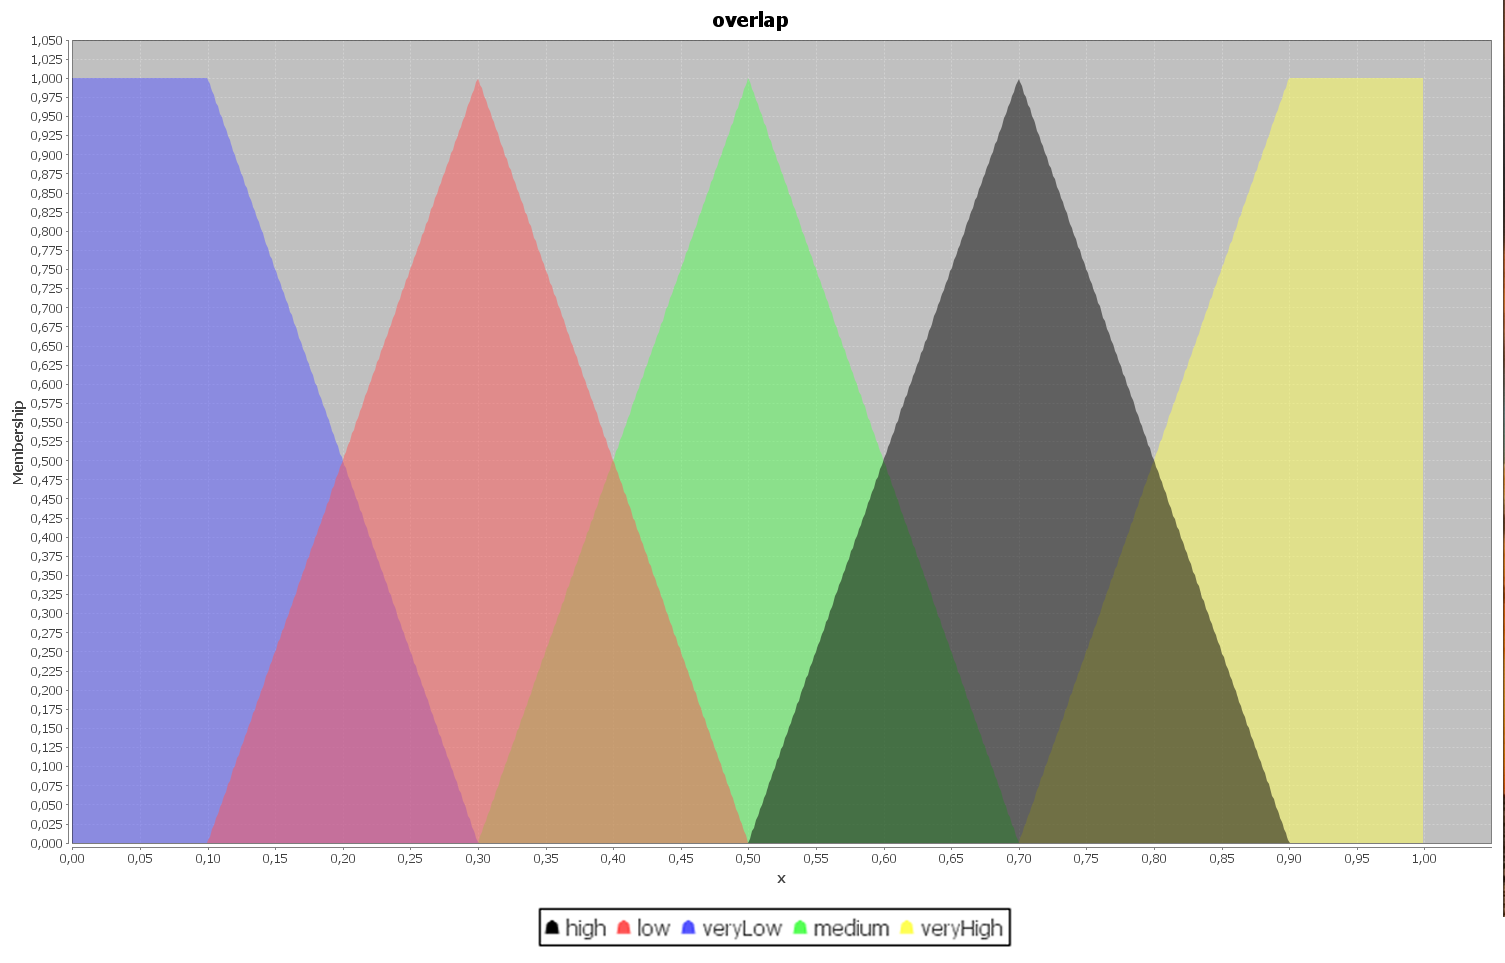
\includegraphics[width=0.9\linewidth]{4_fuzzy-sets-time}
		\caption[Time overlap fuzzy sets]{Time overlap fuzzy sets}
		\label{fig:fs-time}
	\end{figure}

\end{itemize}

Since the above are the input variables taken by the system, the output is given by the \textbf{Modifier} variable, assigned to the fuzzy sets defined in Figure~\ref{fig:fs-modifier}.
	
\begin{figure}
	\centering
	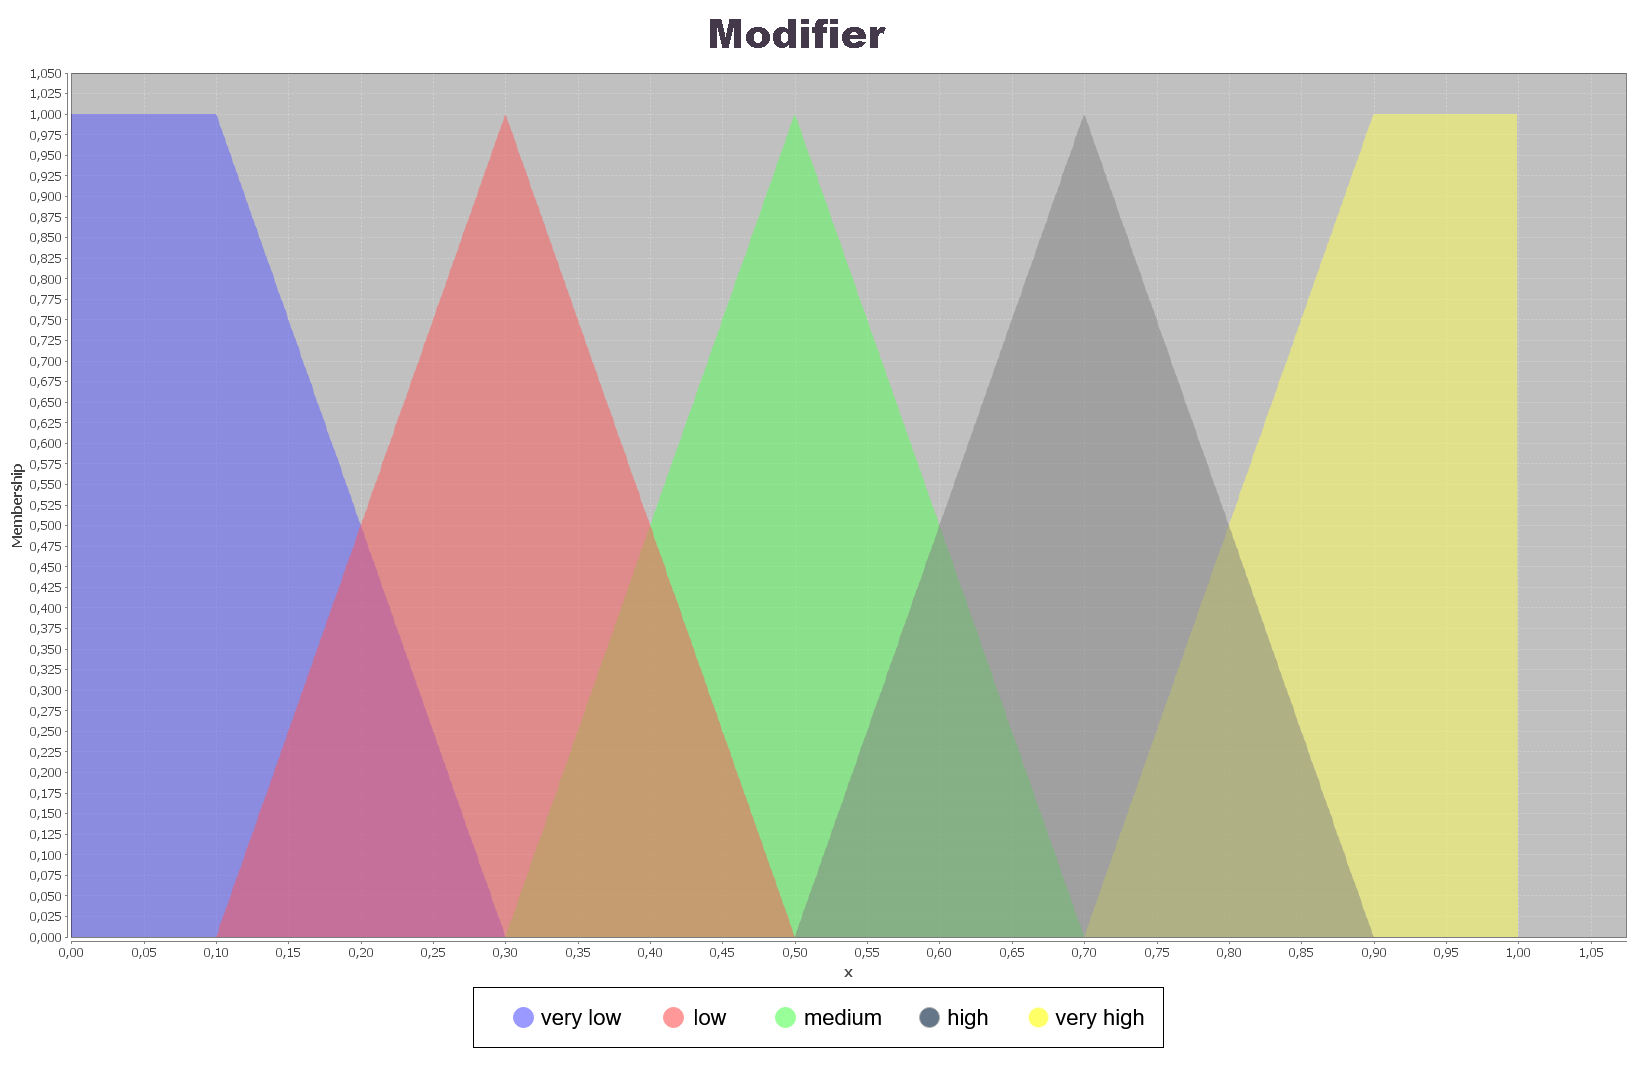
\includegraphics[width=0.9\linewidth]{4_fuzzy-sets-modifier}
	\caption[Weight modifier fuzzy sets]{Weight modifier fuzzy sets}
	\label{fig:fs-modifier}
\end{figure}
	
In turn, the set of rules defined using FCL and used by the system is displayed in Table~\ref{tb:cr-fuzzy-rules}.
	
	\begin{table}
	\centering
	\caption{$C_R$ fuzzy inference system rules}
	\label{tb:cr-fuzzy-rules}
	\resizebox{\textwidth}{!}{%
	\begin{tabular}{|c|l|}
	\hline
	\textbf{N} &
	  \multicolumn{1}{c|}{\textbf{FCL Rule}} \\ \hline\hline
	1 &
	  \begin{tabular}[c]{@{}l@{}}IF (culturalDist IS low OR culturalDist IS veryLow) AND (overlap IS low OR   overlap IS veryLow) \\ AND (englishLevel IS low OR englishLevel IS veryLow) THEN   modifier IS medium;\end{tabular} \\ \hline
	2 &
	  \begin{tabular}[c]{@{}l@{}}IF (culturalDist   IS low OR culturalDist IS veryLow) AND (overlap IS low OR overlap IS veryLow)   \\ AND (englishLevel IS medium OR englishLevel IS high OR englishLevel IS   veryHigh) THEN modifier IS medium;\end{tabular} \\ \hline
	3 &
	  \begin{tabular}[c]{@{}l@{}}IF   (culturalDist IS low OR culturalDist IS veryLow) AND (overlap IS medium) \\ AND (englishLevel IS low OR englishLevel IS veryLow) THEN modifier IS low;\end{tabular} \\ \hline
	4 &
	  \begin{tabular}[c]{@{}l@{}}IF (culturalDist IS low OR culturalDist IS veryLow) AND (overlap IS medium) AND  \\ (englishLevel IS medium OR englishLevel IS high OR englishLevel IS veryHigh) THEN   modifier IS medium;\end{tabular} \\ \hline
	5 &
	  \begin{tabular}[c]{@{}l@{}}IF   (culturalDist IS low OR culturalDist IS veryLow) AND (overlap IS high OR   overlap IS veryHigh) \\ AND (englishLevel IS low OR englishLevel IS veryLow)   THEN modifier IS veryLow;\end{tabular} \\ \hline
	6 &
	  \begin{tabular}[c]{@{}l@{}}IF   (culturalDist IS low OR culturalDist IS veryLow) AND (overlap IS high OR   overlap IS veryHigh) \\ AND (englishLevel IS medium OR englishLevel IS high OR   englishLevel IS veryHigh) THEN modifier IS veryLow;\end{tabular} \\ \hline
	7 &
	  \begin{tabular}[c]{@{}l@{}}IF   (culturalDist IS medium OR culturalDist IS high OR culturalDist IS veryHigh)   \\ AND (overlap IS low OR overlap IS veryLow) AND (englishLevel IS low OR   englishLevel is veryLow) THEN modifier IS veryHigh;\end{tabular} \\ \hline
	8 &
	  \begin{tabular}[c]{@{}l@{}}IF   (culturalDist IS medium OR culturalDist IS high OR culturalDist IS veryHigh)   AND (overlap IS low OR overlap IS veryLow) \\ AND (englishLevel IS medium OR   englishLevel IS high OR englishLevel IS veryHigh) THEN modifier IS high;\end{tabular} \\ \hline
	9 &
	  \begin{tabular}[c]{@{}l@{}}IF   (culturalDist IS medium OR    culturalDist IS high OR culturalDist IS veryHigh) AND (overlap IS   medium) \\ AND (englishLevel IS low OR englishLevel is veryLow) THEN modifier IS   veryHigh;\end{tabular} \\ \hline
	10 &
	  \begin{tabular}[c]{@{}l@{}}IF   (culturalDist IS medium OR culturalDist IS high OR culturalDist IS veryHigh)   AND (overlap IS medium)\\ AND (englishLevel IS medium OR englishLevel IS high   OR englishLevel IS veryHigh) THEN modifier IS medium;\end{tabular} \\ \hline
	11 &
	  \begin{tabular}[c]{@{}l@{}}IF (culturalDist   IS medium OR culturalDist IS high OR culturalDist IS veryHigh) AND (overlap   IS high OR overlap IS veryHigh) \\ AND (englishLevel IS low OR englishLevel is   veryLow) THEN modifier IS high;\end{tabular} \\ \hline
	12 &
	  \begin{tabular}[c]{@{}l@{}}IF   (culturalDist IS medium OR culturalDist IS high OR culturalDist IS veryHigh)   AND (overlap IS high OR overlap IS veryHigh) \\ AND (englishLevel IS medium OR   englishLevel IS high OR englishLevel IS veryHigh) THEN modifier IS medium;\end{tabular} \\ \hline
	\end{tabular}%
	}
	\end{table}

After evaluating the rules, the output modifier produced and conveniently defuzzified by the system will be the value to be added to the original $C_R$ weight. This penalty will attempt to represent the additional communication efforts that must be made between users due to the temporal, geographical and cultural distances between them.

Having studied how this fuzzy inference system works, it will be easily noted how the calculation of the $C_A$ matrix will make use of it in a very similar manner.

\subsubsection{ACTUAL COMMUNICATION MATRIX ($C_A$)}

When representing how users are trying to coordinate, it is necessary to take into account the communications between them. The actual coordination matrix ($C_A$) makes use of the communications within the organization to represent those pairs of users who have communicated, as shown in Figure~\ref{fig:ca-matrix}. Thus, the different cells of the $C_A$ matrix will represent with their weights how much communication has existed between each pair of users in a given project, being these communications related to concrete tasks (see Figure~\ref{fig:ca-class}).

\begin{figure}
	\centering
	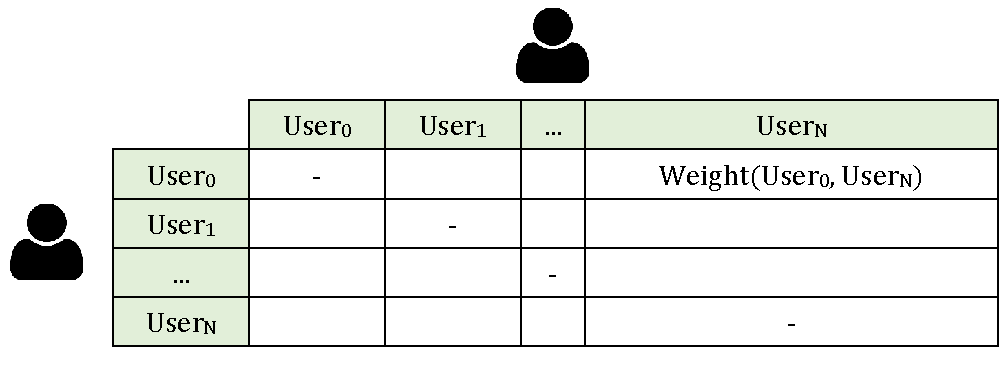
\includegraphics[width=0.95\linewidth]{4_ca-matrix}
	\caption[$C_A$ matrix]{$C_A$ matrix}
	\label{fig:ca-matrix}
\end{figure}

\begin{figure}
	\centering
	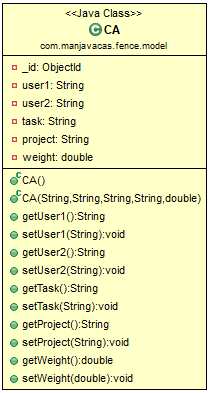
\includegraphics[width=0.32\linewidth]{4_ca-class}
	\caption[$C_A$ class]{$C_A$ class}
	\label{fig:ca-class}
\end{figure}

Before addressing the calculation of the $C_A$ objects stored in the database, it is necessary to clarify how the communications have been obtained to test the algorithm. In order to roughly simulate communications between users in the organization, a Python script was initially used to generate completely random conversations for a given project. However, after multiple iterations it was determined that the generated conversations hardly represented realistic communications, as the number of really useful communications to be generated was simply anecdotal. As a result, the script was consciously modified, giving rise to the one shown in Appendix \ref{cap:annexA}, which in this case did provide more realistic and useful results when testing the tool. As can be seen, the script makes use of the existing coordination requirements in $C_R$ matrix and tries to fulfil them with a random amount of conversations between users. These communications would be stored in the database and used by the $C_A$ matrix algorithm detailed in Algorithm~\ref{alg:ca}.

\begin{algorithm}
    
    \DontPrintSemicolon
    \SetKwInOut{Input}{input}
    \SetKwInOut{Output}{output}
    \Input{project, $C_R$ matrix}
    \Output{$C_A$ matrix}
    
    \caption{$C_A$ calculation}
    \label{alg:ca}
        
        $caMatrix \longleftarrow $\O$ $\;
        $users \longleftarrow getUsers{C_R}()$\;
        
        \ForEach{user $user_1$ in $users$}{
        
            $weight_{C_A} \longleftarrow 0$\;
            $userTasks \longleftarrow getTasksAssignedTo(user_1)$\;
            $userCommunications \longleftarrow getCommunicationsOf(user_1)$\; 
            
            \ForEach{communication $com$ in $userCommunications$}{
            
                $user_2 \longleftarrow getUser_2(com)$\;
                $numDependencies \longleftarrow totalDependencies(user_1,user_2)$\;
                
                \If{numDependencies $>$ 0} {
                
                    $communications \longleftarrow getCommunicationsBetween(user_1,user_2)$\;
                    $totalCommunications \longleftarrow |communications|$\;
                    $taskCommunications \longleftarrow getTaskCommunications(com.task, communications)$\;
                    
                    \;
                    \If{taskCommunications $>$ 0}{
                        
                        \uIf{taskCommunications $\geq$ 5}{
                            $frequency \longleftarrow 1$\;
                        } \uElseIf{taskCommunications $\geq$ 3}{
                            $frequency \longleftarrow 0.6$\;
                        } \uElse{
                            $frequency \longleftarrow 0.3$\;
                        }
                    
                    }\;
                    
                    $weight_{C_A} \mathrel{{+}{=}} (frequency * totalCommunications / numDependencies)$\;
                    $weight_{C_A} \mathrel{{-}{=}} computeGlobalFactors(user_1,user_2)$\;
                    
                    \;
                    \If{$weight_{C_A}$ $>$ 1}{$weight_{C_A}$ $\longleftarrow$ 1}\;
                    
                    $caMatrix \cup C_A(user_1,user_2,com.task,weight_{C_A},project)$\;
                
                }
            
            }
        
        }
    
\end{algorithm}

In this case, the fuzzy inference system is used to adjust the weight obtained. As can be noted, the penalty for temporal, geographical and cultural distances will result in the decrease of the weight, subtracting part of the value of the established communications.

It can also be observed that the calculation of this matrix is the most time-consuming comparing to the other matrices, and that is because the execution of the algorithm depends on relatively large input data, such as users in $C_R$, communications and tasks. However, by following this process, we will have calculated the $C_A$ matrix and will be ready to compare the current communication with the existing coordination requirements.

\subsubsection{COORDINATION GAPS MATRIX ($C_G$)}

The last matrix to be calculated, which will lead us to compute STC, is the coordination gaps matrix ($C_G$). This matrix represents in its cells the difference between the communication that each pair of users must achieve and the communication that is actually taking place (see Figure~\ref{fig:ca-matrix} and Figure~\ref{fig:ca-class}). In other words, each cell of the $C_G$ array for users $user_i$ and $user_j$ represents the difference in weight between $C_R$($user_i$, $user_j$) and $C_A$($user_i$, $user_j$). As can be observed, the weights of the $C_G$ matrix clearly represent the coordination requirements that are being covered as well as those communication gaps that are still present between users.

\begin{figure}
	\centering
	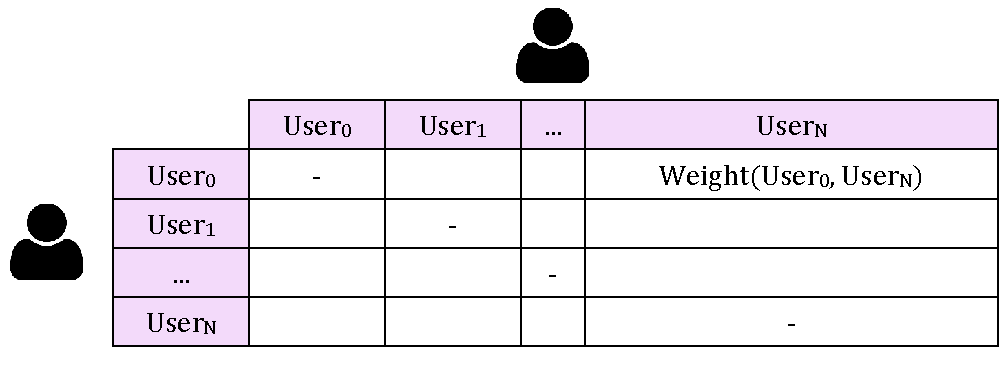
\includegraphics[width=0.95\linewidth]{4_cg-matrix}
	\caption[$C_G$ matrix]{$C_G$ matrix}
	\label{fig:cg-matrix}
\end{figure}

\begin{figure}
	\centering
	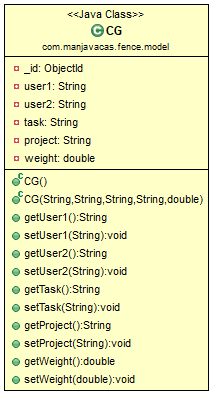
\includegraphics[width=0.32\linewidth]{4_cg-class}
	\caption[$C_G$ class]{$C_G$ class}
	\label{fig:cg-class}
\end{figure}

The procedure followed to fill in this matrix is relatively simple compared to the previous ones, as can be observed in Algorithm~\ref{alg:cg}.

\begin{algorithm}
    
    \DontPrintSemicolon
    \SetKwInOut{Input}{input}
    \SetKwInOut{Output}{output}
    \Input{$C_A$ matrix, $C_R$ matrix}
    \Output{$C_G$ matrix}
    
    \caption{$C_G$ calculation}
    \label{alg:cg}
        
        $cgMatrix \longleftarrow $\O$ $\;
       
        \ForEach{$cr$ in $crMatrix$}{
            $caList \longleftarrow getCA(cr.user_1,cr.user_2,cr.project,cr.task)$\;
            
            \uIf{caList $\ne$ \O}{
               $weight_{C_A} \longleftarrow sumWeights(caList)$\;
               $weight_{C_R} \longleftarrow cr.weight$\;
               $weight_{C_G} \longleftarrow weight_{C_R} - weight_{C_A}$\;
               
               \If{$weight_{C_G}$ $>$ 0} {
                    $cgMatrix \cup C_G(cr.user_1, cr.user_2, cr.task, weight_{C_G}, cr.project)$\;
               }
            }\Else{
                $cgMatrix \cup C_G(cr.user_1, cr.user_2, cr.task, cr.weight, cr.project)$\;
            }
        }
    
\end{algorithm}

With the $C_G$ matrix representing the lack of coordination between users in a given project, the calculation of the organisation's STC levels will then be undertaken.

\subsubsection{SOCIOTECHNICAL CONGRUENCE MEASUREMENT}

As we have already indicated, the requirements to be met by FENCE involve the calculation of STC levels from three different points of view: employees, teams, and projects. As we shall see below, knowing the STC level of the organisation's teams and projects is relatively simple, being the obtainment of the employees' STC levels the basis of this calculations.

\begin{itemize}
\item \textbf{Employees' STC}
\end{itemize}

To calculate the individual STC of each user we will follow the process detailed in Algorithm~\ref{alg:stc-user}, where Equation~\ref{eq:stc-user} will be used to calculate the individual level of STC for each employee.

\begin{algorithm}
    
    \DontPrintSemicolon
    \SetKwInOut{Input}{input}
    \SetKwInOut{Output}{output}
    \Input{project, $C_R$ Matrix, $C_G$ matrix}
    \Output{users STC}
    
    \caption{User STC calculation}
    \label{alg:stc-user}
        
        $stcUsers \longleftarrow $\O$ $\;
        $users \longleftarrow getProjectUsers(project)$\;
        
        \ForEach{$user$ in $users$}{
            $userCRs \longleftarrow getUserCRs(user)$\;
            $userCGs \longleftarrow getUserCGs(user)$\;
            
            $userCRsum \longleftarrow sumWeights(userCRs)$\;
            $userCGsum \longleftarrow sumWeights(userCGs)$\;
            
            \uIf{userCGsum $\leq$ 0} {
                $stcUsers \cup UserSTC(user, 100.0, getCurrentDate())$\;
            }\Else{
                $stcUser \longleftarrow 1 - (userCGsum / userCRsum)$\;
                $stcUsers \cup UserSTC(user, stcUser * 100, getCurrentDate())$\;
            }
        }
        
\end{algorithm}


\begin{equation}
\label{eq:stc-user}
STC = 1 - \frac{\sum_{i=0}^{n}\sum_{j=0}^{n}C_{Gij}}{\sum_{i=0}^{n}\sum_{j=0}^{n}C_{Rij}}
\end{equation}

At the same time, note how each measurement will be dated. This will allow us to have a history of the STC levels for each user, team, and project, whose usefulness will be seen in the next module.

\begin{itemize}
\item \textbf{Teams' STC}
\end{itemize}

In this case, as shown in Algorithm~\ref{alg:stc-team}, the calculation of the STC at team level is very similar to the previous one, except that the users considered are those belonging to the chosen team.

\begin{algorithm}
    
    \DontPrintSemicolon
    \SetKwInOut{Input}{input}
    \SetKwInOut{Output}{output}
    \Input{project, $C_R$ Matrix, $C_G$ matrix}
    \Output{teams STC}
    
    \caption{Teams STC calculation}
    \label{alg:stc-team}
        
        $stcTeams \longleftarrow $\O$ $\;
        $teams \longleftarrow getProjectTeams(project)$\;
        
        \ForEach{$team$ in $teams$}{
            $teamCRsum \longleftarrow 0 $\;
            $teamCGsum \longleftarrow 0 $\;
            $teamUsers \longleftarrow team.users$\;
            
            \ForEach{$user$ in $teamUsers$}{
            
                $userCRs \longleftarrow getUserCRs(user)$\;
                $userCGs \longleftarrow getUserCGs(user)$\;
                
                $teamCRsum \mathrel{{+}{=}} sumWeights(userCRs)$\;
                $teamCGsum \mathrel{{+}{=}} sumWeights(userCGs)$\;
                
            }  
            
            \uIf{teamCGsum $\leq$ 0} {
                $stcTeams \cup TeamSTC(team, 100.0, getCurrentDate())$\;
            }\Else{
                $stcTeam \longleftarrow 1 - (teamCGsum / teamCRsum)$\;
                $stcTeams \cup TeamSTC(team, stcTeam * 100, getCurrentDate())$\;
            }
        }  
    
    \end{algorithm}

As in the previous case, we will keep a history of the STC measurements for teams.

\begin{itemize}
\item \textbf{Project STC}
\end{itemize}

Having calculated the STC at user and team level, it only remains to measure it at project level by following the process detailed in Algorithm~\ref{alg:stc-project}.

\begin{algorithm}
    
    \DontPrintSemicolon
    \SetKwInOut{Input}{input}
    \SetKwInOut{Output}{output}
    \Input{project, $C_R$ Matrix, $C_G$ matrix}
    \Output{project STC}
    
    \caption{Project STC calculation}
    \label{alg:stc-project}
        
        $projectCRsum \longleftarrow sumWeights(C_R)$\;
        $projectCGsum \longleftarrow sumWeights(C_G)$\;
        
        \uIf{projectCGsum $\leq$ 0} {
            $stcProject \cup ProjectsSTC(team, 100.0, getCurrentDate())$\;
        }\Else{
            $stcProject \longleftarrow 1 - (projectCGsum / projectCRsum)$\;
            $stcProject \cup ProjectSTC(project, stcProject * 100, getCurrentDate())$\;
        }
        
    \end{algorithm}

Once seen in detail the implementation of the algorithms and their adaptation to the information handled by FENCE, it only remains to illustrate how the information is requested by the user and displayed in the interface (see Figure~\ref{fig:stc-measurer}).

\begin{figure}
	\centering
	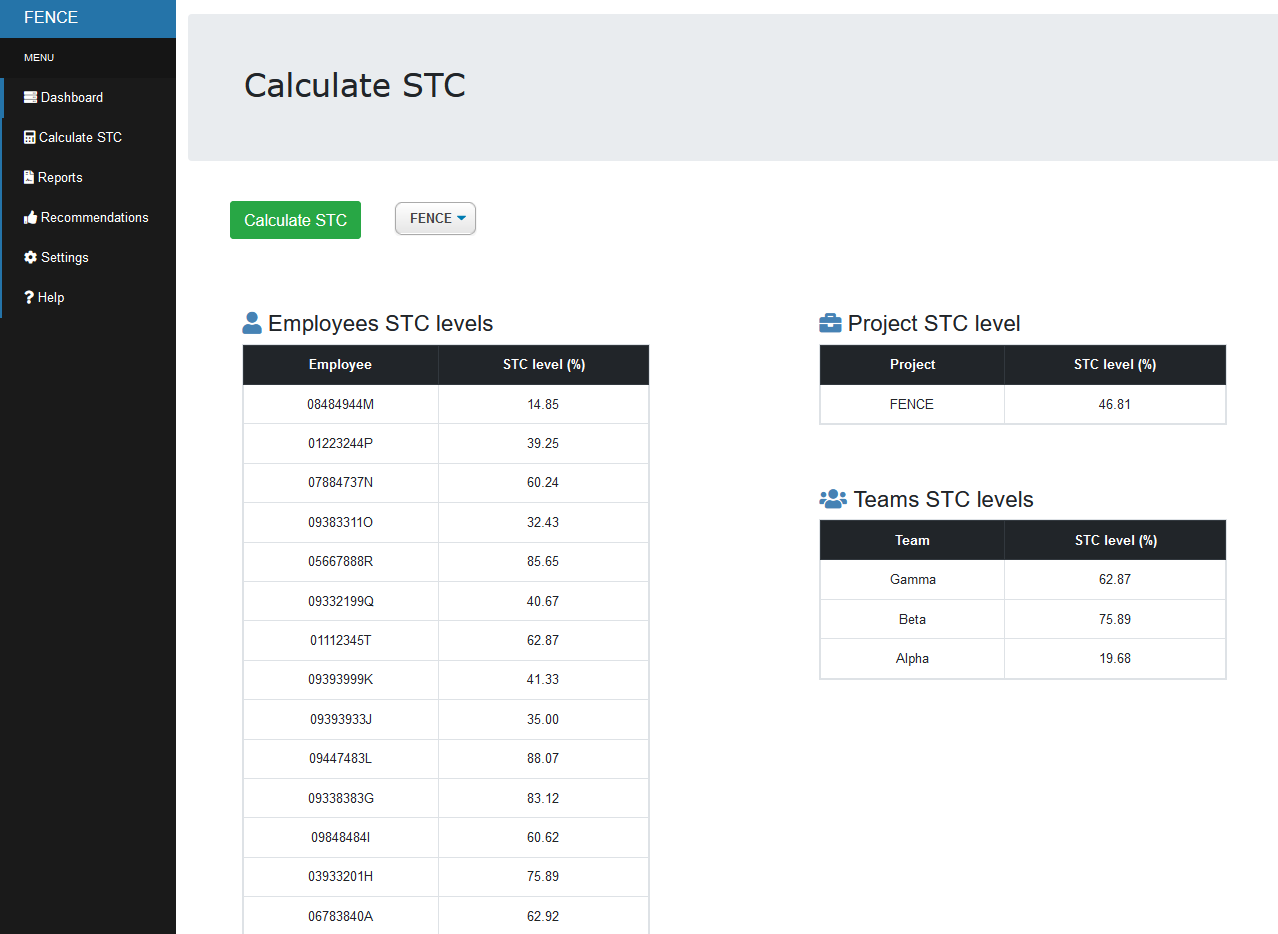
\includegraphics[width=0.95\linewidth]{4_stc-measurer}
	\caption[STC measurer interface]{STC measurer interface}
	\label{fig:stc-measurer}
\end{figure}

\begin{itemize}
\item Initially, when the user accesses the STC tab, the last measurements made by the tool will be loaded into the different tables: users, teams, and project tables. 
\item If the user wants to recalculate the STC levels for a given project, he or she must select it and directly click on the "Calculate STC" button. 
\item This will cause the STC levels to be recalculated, along with the values from the different matrices, being also updated in the database. 
\item Finally, once this process is completed, the tables will be filled with the most updated version of the STC levels.
\end{itemize}

As can be noted, new resources such as classes to model STC measurements and matrices were included and implemented in this phase, while others previously defined were expanded or adjusted to the needs of the STC meter.

It also should be considered that the entire execution of the STC calculation algorithm is quite computational costly. Although this complexity was iteratively reduced, resulting in significantly better performance, the amount of time required for execution remained considerable given the complexity of the calculations to be made and the number of inputs (users, tasks, assignments, dependencies, communications) to be handled.

Nevertheless, the results provided by the system developed in this module would serve as a basis for the development and use of the following modules, focused on visualizing and improving the organization's STC levels.

\subsection{Module 4. Data visualization}

The objective of the work carried out in this module was to allow the visualization of time series with information on STC measurements in employees, teams, and projects. Based on this, the implementation of the graphics was carried out using the JavaScript library \emph{Chart.js}.

This library offers a flexible and simple way to generate many types of charts. In this case, the input data would be displayed in a timeline, corresponding to the latest STC measurements for each employee, team, and project.

Looking at the FENCE interface, as can be seen in Figure~\ref{fig:reports}, the user will find three canvas with which he or she can interact by selecting at convenience the specific employee, team or project from which it is desired to know its STC history levels.

\begin{figure}
	\centering
	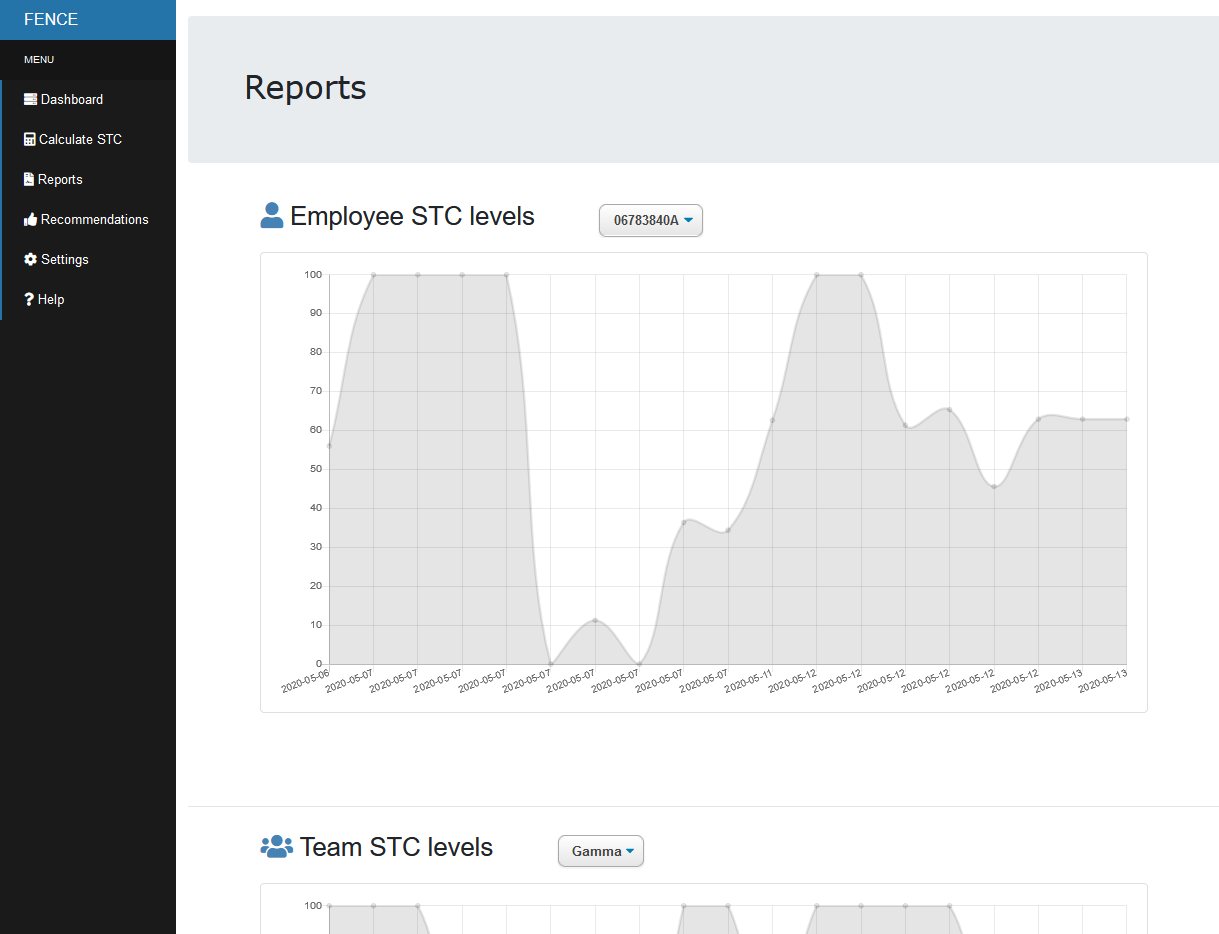
\includegraphics[width=0.95\linewidth]{4_reports}
	\caption[Reports interface]{Reports interface}
	\label{fig:reports}
\end{figure}

If we go deeper into the construction and operation of the charts beyond the interface, initially the application makes GET-type Ajax requests to the corresponding controllers. Each controller shown in Figure~\ref{fig:measurements-controllers} receives the request and invokes the corresponding method in the associated service object (see Figure~\ref{fig:measurements-services}), which retrieves and returns all the measurements stored in the database. When each Ajax request receives the result of the query, the last 20 measurements performed are extracted and entered as input data to be represented by the \emph{Chart.js} plot.

\begin{figure}
	\centering
	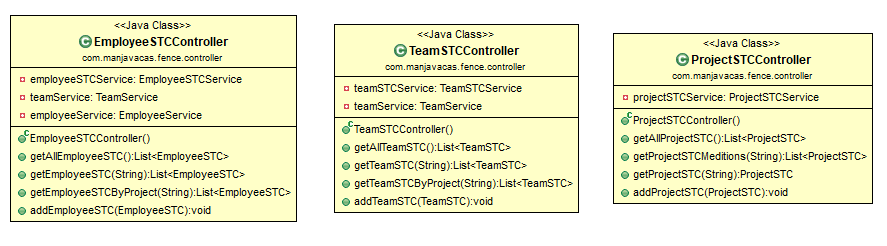
\includegraphics[width=0.95\linewidth]{4_controllers-measurement}
	\caption[STC measurements controllers]{STC measurements controllers}
	\label{fig:measurements-controllers}
\end{figure}

\begin{figure}
	\centering
	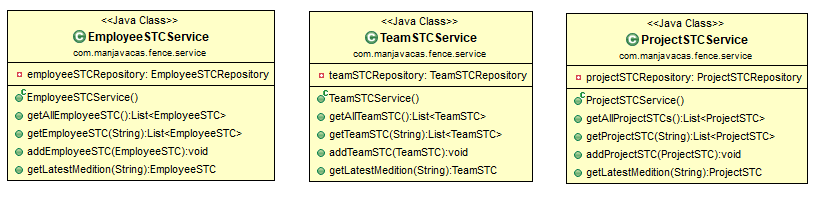
\includegraphics[width=0.95\linewidth]{4_services-measurement}
	\caption[STC measurements services]{STC measurements services}
	\label{fig:measurements-services}
\end{figure}

This is a fast and simple process, which provides FENCE with more analytical capabilities for the analysis of STC levels evolution. Visualising this progression can help project managers, or even strategic leaders, to consider what issues are affecting the performance of the global projects. 

Once this phase based on data visualisation has been overcome, the next module would allow to undertake concrete actions to improve the STC levels within the organisation.

\subsection{Module 5. Recommendation system}

This module addressed the development of one of the main and most distinctive functionalities of FENCE: the development of a recommendation system focused on providing information to the user about how to improve the STC levels of the organization.

Before starting the development of this system, meetings were held with the different stakeholders:

\subsubsection{TECHNICAL PLANNING}
Initially, it was discussed through different meetings with José Ángel Olivas how to approach the development of the recommendation system by using the information provided by FENCE. It was agreed that the coordination gap matrix ($C_G$) was ideal for finding out which users were those on whom recommendations should be made. Moreover, the variables and rules to be used by the fuzzy inference system were also studied and initially outlined.

After these sessions, multiple alternatives were considered when working with fuzzy logic in Java, being finally jFuzzyLogic \cite{cingolani_jfuzzylogic_2012, cingolani_jfuzzylogic_2013} the library chosen for this task. This library is based on the definition of fuzzy inference systems by means of the standard FCL \cite{FCL}, so it was necessary to learn its syntax in the handling of variables, functions, fuzzy sets, and rules.

The main features of this library that led to its use were: its flexibility and ease of integration with the system developed so far; the use of FCL (a relatively simple fuzzy definition language) as well as being quite updated in relation to other fuzzy logic libraries found.

With this technical base and once familiar with jFuzzyLogic after multiple tests, the Knowledge Engineering work was carried out together with the Aurora Vizcaíno, who played the role of expert.

\subsubsection{KNOWLEDGE ENGINEERING}

Knowledge Engineering involves the extraction of expert knowledge and its translation into a formalized language in a precise, unambiguous, and exploitable way. On this basis, the Knowledge Engineering tasks performed would allow us to define the features that should be covered by the recommending system. 

If we study its scope and limitations, the following ones were considered:

\begin{itemize}
	\item \textbf{Scope}: given the characteristics of the users that integrate the multiple teams on a given project, as well as the organization's STC levels, the system will offer as output recommendations to improve those STC levels in a clear and traceable way.
	\item \textbf{Limitations}: the number of features covered will be strictly limited to the knowledge of the expert. The system shall also not contemplate specific features of the project, teams and users going beyond the information provided as input.
\end{itemize}

Subsequently, once the domain of the system had been established, the choice of the expert willing to transmit her knowledge was made. In this case, as previously stated, it was Aurora Vizcaíno, university professor and researcher in the Computer Science School of Ciudad Real. It was considered that her contributions would be an important source of knowledge given her experience in the field of GSD, as well as her work in multiple research projects related to communication and knowledge management in this domain.

On the other hand, one of the main tasks of the knowledge engineer is the study of the viability of the project to be undertaken. An effective method for this purpose is the Slagel Test \cite{mate_1998}, which is focused on the study of the plausibility, justification, success, adequacy, and success of expert systems, allowing to determine if the project is viable based on the reasoning over its characteristics:

\begin{itemize}
\item \textbf{Plausibility}: determines whether the necessary means to address the problem from the perspective of Knowledge Engineering are available. From this point of view, the characteristics of the expert and the task to be undertaken are analysed.
\item \textbf{Justification}: analysis of the need for experience and the investment to be made (type of environment, need due to volatile experience, return of investment, alternative solutions, etc.).
\item \textbf{Adequacy}: it is studied if the problem is adequate to be solved with Knowledge Engineering techniques, analysing its nature, complexity, and type.
\item \textbf{Success}: the probabilities of the system's success are determined in advance. It involves studying non-technical but important issues in order to decide to apply Knowledge Engineering to the resolution of the problem, such as the involvement and responsibility of the people implicated, as well as the acceptance of the system in its environment.
\end{itemize}

In this way, the process conducted in order to justify the viability of the recommending system to be developed is shown below:

\begin{itemize}
\item First, for each of the dimensions mentioned, three different categories are established:

	\begin{itemize}
	\item Managers and/or users (MU).
	\item Experts (EX).
	\item Tasks (TA).
	\end{itemize}

	\vspace{2mm}

	For each category, the most important features that define that dimension are specified. These features may be essential (E) or desirable (D), considering that essential features must not have a value below a threshold (7 in this case).

	\vspace{2mm}

	On this basis, each feature is assigned a weight between 0 and 10, depending on its relative importance. This entire process is summarized in tables Table \ref{tb:plau}, Table \ref{tb:just}, Table \ref{tb:adeq}, and Table \ref{tb:suc}.\newline

\begin{table}[]
	\centering
	\caption[Plausability study]{Plausability study}
	\label{tb:plau}
	\resizebox{\textwidth}{!}{%
	\begin{tabular}{|c|c|c|c|l|c|}
	\hline
	\multicolumn{6}{|c|}{\textbf{Plausibility}} \\ \hline\hline
	\textbf{Category} &
	  \textbf{Identifier} &
	  \textbf{Weight} &
	  \textbf{Value} &
	  \multicolumn{1}{c|}{\textbf{Feature definition}} &
	  \textbf{Type} \\ \hline\hline
	EX &
	  P1 &
	  10 &
	  8 &
	  Experts    exist &
	  E \\ \hline
	EX &
	  P2 &
	  10 &
	  9 &
	  The    assigned expert is genuine &
	  E \\ \hline
	EX &
	  P3 &
	  8 &
	  10 &
	  The    expert is cooperative &
	  D \\ \hline
	EX &
	  P4 &
	  7 &
	  9 &
	  \begin{tabular}[c]{@{}l@{}}The expert    is able to articulate his/her methods, \\ but does not categorize\end{tabular} &
	  D \\ \hline
	TA &
	  P5 &
	  10 &
	  8 &
	  There    are enough test cases &
	  E \\ \hline
	TA &
	  P6 &
	  10 &
	  9 &
	  The    task is well structured and understood &
	  D \\ \hline
	TA &
	  P7 &
	  10 &
	  8 &
	  It    only requires cognitive ability &
	  D \\ \hline
	TA & P8 & 9 & 8 & \begin{tabular}[c]{@{}l@{}}No    optimal results are required but only satisfactory ones, \\ without    compromising the project\end{tabular} & D \\ \hline
	TA &
	  P9 &
	  9 &
	  7 &
	  The    task does not require common sense &
	  D \\ \hline
	DU &
	  P10 &
	  7 &
	  10 &
	  The    managers are truly committed to the project &
	  D \\ \hline
	\end{tabular}%
	}
\end{table}

\begin{table}[]
	\centering
	\caption[Justification study]{Justification study}
	\label{tb:just}
	\resizebox{\textwidth}{!}{%
	\begin{tabular}{|c|c|c|c|l|c|}
	\hline
	\multicolumn{6}{|c|}{\textbf{Justification}}                                        \\ \hline\hline
	\textbf{Category} &
	  \textbf{Identifier} &
	  \textbf{Weight} &
	  \textbf{Value} &
	  \multicolumn{1}{c|}{\textbf{Feature definition}} &
	  \textbf{Type} \\ \hline\hline
	EX & J1 & 10 & 9 & The expert is   not available                                & E \\ \hline
	EX & J2 & 10 & 9 & There's a   shortage of human experience                     & D \\ \hline
	TA & J3 & 8  & 9 & There is a   need for simultaneous experience in many places & D \\ \hline
	TA &
	  J4 &
	  10 &
	  8 &
	  \begin{tabular}[c]{@{}l@{}}Need for   experience in hostile, distressing and/or \\ unrewarding environments\end{tabular} &
	  E \\ \hline
	TA & J5 & 8  & 9 & There are no   admissible alternative solutions              & E \\ \hline
	MU & J6 & 7  & 9 & A high rate of   return on investment is expected            & D \\ \hline
	MU & J7 & 8  & 9 & Solves a   useful and necessary task                         & E \\ \hline
	\end{tabular}%
	}
\end{table}

\begin{table}[]
	\centering
	\caption[Adequacy study]{Adequacy study}
	\label{tb:adeq}
	\resizebox{\textwidth}{!}{%
	\begin{tabular}{|c|c|c|c|l|c|}
	\hline
	\multicolumn{6}{|c|}{\textbf{Adequacy}}                                          \\ \hline\hline
	\textbf{Category} &
	  \textbf{Identifier} &
	  \textbf{Weight} &
	  \textbf{Value} &
	  \multicolumn{1}{c|}{\textbf{Feature definition}} &
	  \textbf{Type} \\ \hline\hline
	EX & A1  & 5 & 7  & The expert's   experience is poorly organized            & D \\ \hline
	TA & A2  & 6 & 7  & It has little   practical value                          & D \\ \hline
	TA & A3  & 7 & 7  & It is a more   tactical than strategic task              & D \\ \hline
	TA & A4  & 7 & 9  & The task   provides solutions that serve long-term needs & E \\ \hline
	TA &
	  A5 &
	  5 &
	  9 &
	  \begin{tabular}[c]{@{}l@{}}The task is   not too easy, but it is knowledge-intensive, \\ both in the domain and in the   manipulation of information\end{tabular} &
	  D \\ \hline
	TA &
	  A6 &
	  6 &
	  9 &
	  \begin{tabular}[c]{@{}l@{}}It is   manageable in size, and/or a gradual approach is possible and/or, \\ a breakdown   into independent sub-tasks\end{tabular} &
	  D \\ \hline
	EX & A7  & 7 & 10 & The transfer   of experience between humans is feasible  & E \\ \hline
	TA &
	  A8 &
	  6 &
	  9 &
	  \begin{tabular}[c]{@{}l@{}}It was   identified as a problem in the area and the effects of introducing \\ an expert   system can be planned\end{tabular} &
	  D \\ \hline
	TA & A9  & 9 & 10 & No   "immediate" real-time answers required              & E \\ \hline
	TA & A10 & 9 & 8  & The task does   not require basic research               & E \\ \hline
	TA &
	  A11 &
	  5 &
	  7 &
	  The expert basically   uses symbolic reasoning involving subjective factors &
	  D \\ \hline
	TA & A12 & 5 & 9  & It is   essentially heuristic                            & D \\ \hline
	\end{tabular}%
	}
\end{table}

\begin{table}[]
	\centering
	\caption[Success study]{Success study}
	\label{tb:suc}
	\resizebox{\textwidth}{!}{%
	\begin{tabular}{|c|c|c|c|l|c|}
	\hline
	\multicolumn{6}{|c|}{\textbf{Success}}                                                                \\ \hline\hline
	\textbf{Category} &
	  \textbf{Identifier} &
	  \textbf{Weight} &
	  \textbf{Value} &
	  \multicolumn{1}{c|}{\textbf{Feature definition}} &
	  \textbf{Type} \\ \hline\hline
	EX &
	  E1 &
	  8 &
	  10 &
	  \begin{tabular}[c]{@{}l@{}}Users do not   feel threatened by the project, they are able to feel\\ intellectually attached   to the project\end{tabular} &
	  D \\ \hline
	EX & E2  & 6 & 9  & Users have a   remarkable track record in performing this task                & D \\ \hline
	EX & E3  & 5 & 9  & There are   agreements on what constitutes a good solution to the task        & D \\ \hline
	EX &
	  E4 &
	  5 &
	  9 &
	  \begin{tabular}[c]{@{}l@{}}The only   justification for taking a step in the solution is the \\ quality of the final   solution\end{tabular} &
	  D \\ \hline
	EX & E5  & 6 & 8  & There is no   strict deadline, nor does any other project depend on this task & D \\ \hline
	TA & E6  & 7 & 10 & It is not   influenced by politics                                            & E \\ \hline
	TA & E7  & 8 & 7  & Expert systems   already exist to solve this or similar tasks                 & D \\ \hline
	TA & E8  & 8 & 8  & There are   minimal changes to standard procedures                            & D \\ \hline
	TA & E9  & 5 & 9  & Solutions are   explainable or interactive                                    & D \\ \hline
	TA & E10 & 7 & 8  & The task is   one of practical R\&D, but not both simultaneously              & E \\ \hline
	MU &
	  E11 &
	  6 &
	  9 &
	  \begin{tabular}[c]{@{}l@{}}Users are   mentally sound and have realistic expectations \\ of both the scope and   limitations\end{tabular} &
	  D \\ \hline
	MU & E12 & 7 & 9  & They do not   reject this technology out of hand                              & E \\ \hline
	MU & E13 & 6 & 9  & The system   interacts intelligently and friendly with the user               & D \\ \hline
	MU & E14 & 9 & 8  & The system is   able to explain to the user its reasoning                     & D \\ \hline
	MU &
	  E15 &
	  8 &
	  9 &
	  \begin{tabular}[c]{@{}l@{}}The insertion   of the system takes place without injuries; it hardly interferes \\ with the   daily routine of the company\end{tabular} &
	  D \\ \hline
	MU &
	  E16 &
	  6 &
	  9 &
	  \begin{tabular}[c]{@{}l@{}}Users are   committed for the entire duration of the project,\\ even after its   implementation\end{tabular} &
	  D \\ \hline
	MU & E17 & 8 & 9  & Adequate   technology transfer takes place                                    & E \\ \hline
	\end{tabular}%
	}
\end{table}

\item Once the values have been assigned, we proceed as follows:

	\begin{itemize}
	\item If the value of an essential feature does not reach the required threshold, it is counted as 0 and the application is rejected.
	\item Otherwise, we multiply the values of each feature by its corresponding weight to obtain their pondered values.
	\item We then multiply these pondered values for each dimension.
	\item Finally, we compute the geometric pseudo-mean of the weighted values for each dimension, as shown in Equation \ref{eq:plau}, Equation \ref{eq:just}, Equation \ref{eq:adeq}, and Equation \ref{eq:succ}.
	\end{itemize}
	
\begin{equation}
\label{eq:plau}
VC_1 = \prod_{i=1,2,5}^{}\left \lfloor \frac{V_{pi}}{V_{ui}} \right \rfloor (\prod_{i=1}^{10}P_{pi} * V_{pi})^\frac{1}{10} = 76.01
\end{equation}

\begin{equation}
\label{eq:just}
VC_2 = \prod_{i=1,4,5,7}^{}\left \lfloor \frac{V_{ji}}{V_{ui}} \right \rfloor (\prod_{i=1}^{10}P_{ji} * V_{ji})^\frac{1}{7} = 76.43
\end{equation}

\begin{equation}
\label{eq:adeq}
VC_3 = \prod_{i=4,7,9,10}^{}\left \lfloor \frac{V_{ai}}{V_{ui}} \right \rfloor (\prod_{i=1}^{10}P_{ai} * V_{ai})^\frac{1}{12} = 52.37
\end{equation}

\begin{equation}
\label{eq:succ}
VC_4 = \prod_{i=6,10,12,17}^{}\left \lfloor \frac{V_{pi}}{V_{ui}} \right \rfloor (\prod_{i=1}^{17}P_{ei} * V_{ei})^\frac{1}{17} = 57.57
\end{equation}

\item Finally, we compute the normalized mean of the weights of all the dimensions, as shown in Equation \ref{eq:vc} and Equation \ref{eq:vcnorm}, resulting in a percentage that reflects the viability of the system (Table \ref{tb:viability}):


\begin{equation}
\label{eq:vc}
VC = \frac{VC_1 + VC_2 + VC_3 + VC_4}{4} = \frac{76.01 + 76.43 + 52.37 + 57.57}{4} = 65.6
\end{equation}

\begin{equation}
\label{eq:vcnorm}
VC_{norm} = \frac{VC * 100}{Max.VC} = \frac{65.6 * 100}{76.1237} = 86.18 %
\end{equation}

\begin{table}[]
	\centering
	\caption{Viability of the system}
	\label{tb:viability}
	\begin{tabular}{|c|c|c|c|}
	\hline
	\textbf{Category} & \textbf{Rate} & \textbf{Mean viability rate} & \textbf{Normalized viability rate} \\ \hline\hline
	VC1               & 76,01         & \multirow{4}{*}{$VC$ = 65.6}   & \multirow{4}{*}{$VC_{norm}$ = 86.18 \%} \\ \cline{1-2}
	VC2 & 76,43 &  &  \\ \cline{1-2}
	VC3 & 52,37 &  &  \\ \cline{1-2}
	VC4 & 57,57 &  &  \\ \hline
	\end{tabular}
\end{table}

\end{itemize}

With a viability rate of 86.18\%, the proposal was considered viable and, therefore, its development was undertaken.

The next step was the acquiring of expert knowledge, whose extraction was carried out by means of structured interviews agreed upon with the expert. In these meetings, the solutions that the system should provide to different types of situations presented by the interviewer were discussed, as well as the different variables and values that would be translated into fuzzy system inputs.

A total of three meetings made it possible to refine the knowledge obtained, and thus establish the basis for the recommendation system to be developed.

\subsubsection{EXPERT SYSTEM DEVELOPMENT}

With the expert knowledge formalized and translated into rules, the implementation of the system was addressed. First, we will see the variables considered and their corresponding fuzzy sets:

\paragraph{a) Input variables}

\begin{itemize}
\item \textbf{Cultural distance}. Average of the distances between socio-cultural factors identified by \cite{hofstede_cultures_2004} according to the nationality of the users. Calculated as already shown in the $C_R$ matrix explanation of section \ref{sec:stc}, with the same fuzzy sets.
\item \textbf{Time overlap}.  Coincidence between employees’ time zones (UTC), calculated as the inverse of their time difference. A greater time overlap will facilitate the use of synchronous means of communication, while the impossibility of temporal coincidence in communication will result in greater use of asynchronous means. As in the previous case, this input parameter was already defined in section \ref{sec:stc}.
\item \textbf{English level}. Level of English shared by users. The method for obtaining this value and its fuzzy sets was also defined in section \ref{sec:stc}.
\item \textbf{Age1}, \textbf{Age2}. Age of the evaluated employees, represented by the fuzzy sets in Figure \ref{fig:fs-age}.

	\begin{figure}
		\centering
		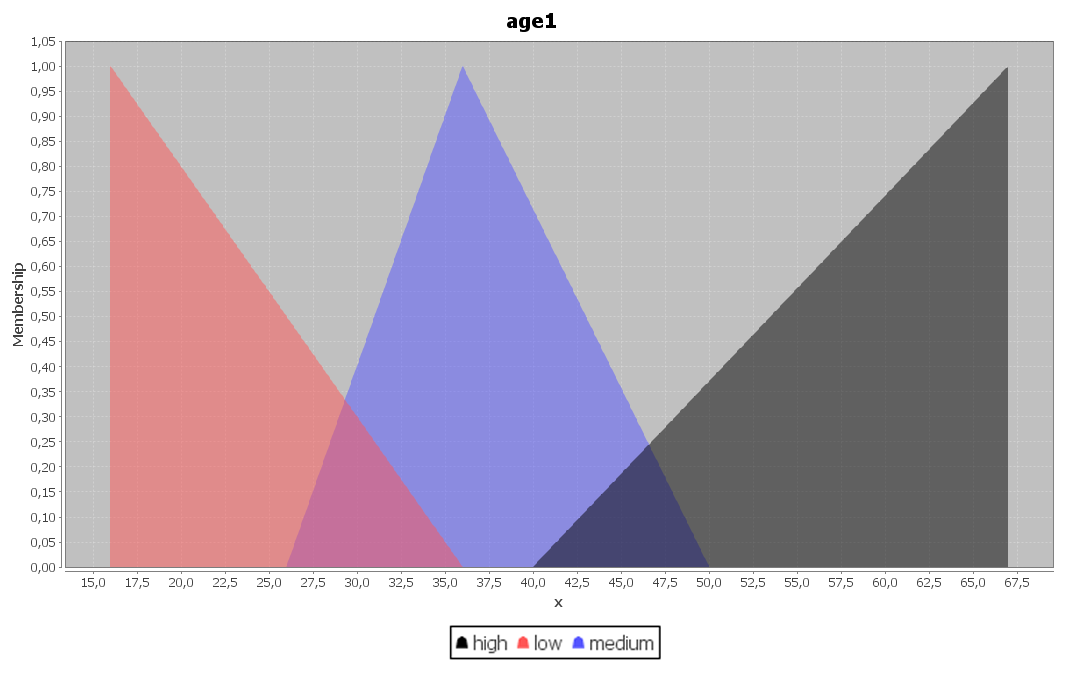
\includegraphics[width=0.9\linewidth]{4_fuzzy-sets-age}
		\caption[Age fuzzy sets]{Age fuzzy sets}
		\label{fig:fs-age}
	\end{figure}

\item \textbf{Experience1}, \textbf{Experience2}. Individual user work experience, whose levels are depicted in Figure \ref{fig:fs-exp}.
\end{itemize}

	\begin{figure}
		\centering
		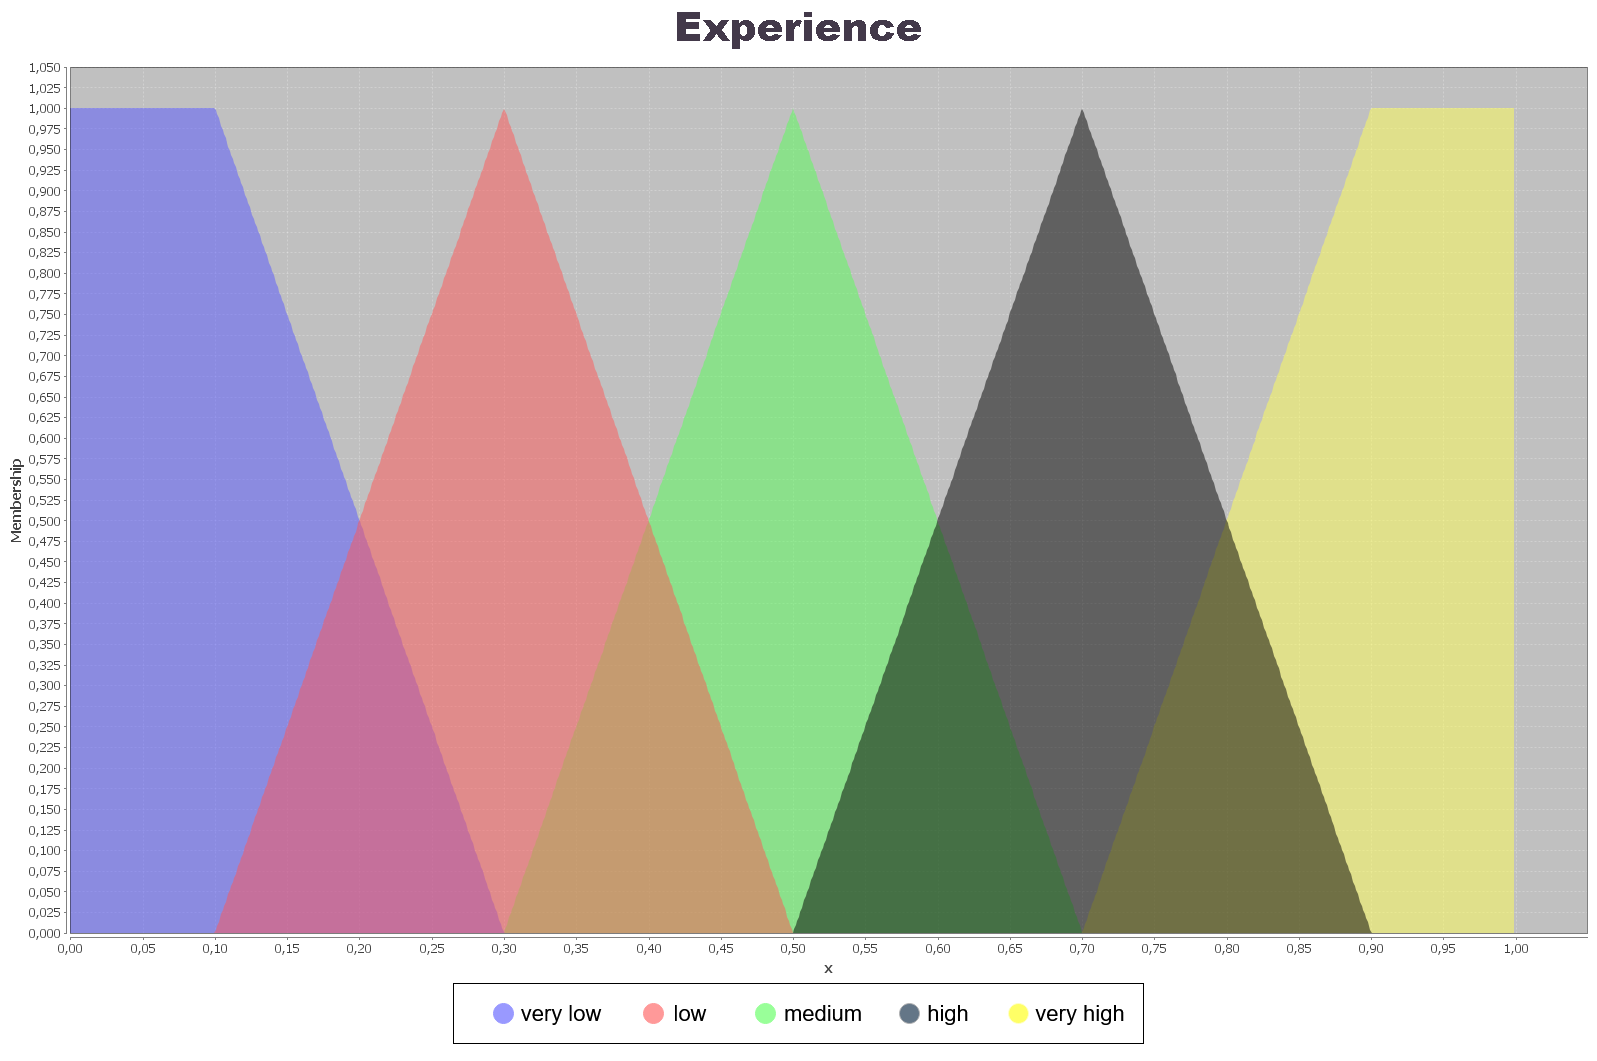
\includegraphics[width=0.9\linewidth]{4_fuzzy-sets-experience}
		\caption[Experience fuzzy sets]{Experience fuzzy sets}
		\label{fig:fs-exp}
	\end{figure}

\paragraph{b) Output variables}

\begin{itemize}
\item \textbf{Mediator}. Indicates whether a mediator is needed if there is a high cultural distance between users. It is a singleton set with singleton centre of gravity (COGS) as defuzzification method, as shown in Figure \ref{fig:fs-mediator}.

	\begin{figure}
		\centering
		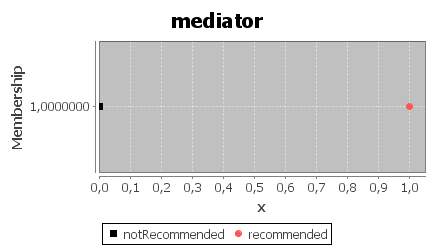
\includegraphics[width=0.6\linewidth]{4_fuzzy-sets-mediator}
		\caption[Mediator singleton fuzzy sets]{Mediator singleton fuzzy sets}
		\label{fig:fs-mediator}
	\end{figure}

\item \textbf{Training}. Represents the need for cultural training when the cultural distance between individuals is medium or moderate. This is another singleton set (see Figure \ref{fig:fs-train}) with COGS as a defuzzification method.

	\begin{figure}
		\centering
		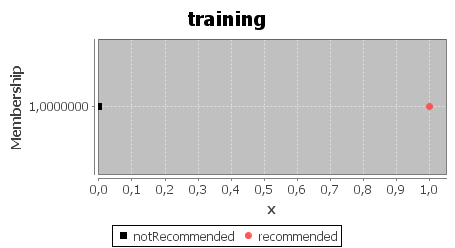
\includegraphics[width=0.6\linewidth]{4_fuzzy-sets-training}
		\caption[Training singleton fuzzy sets]{Training singleton fuzzy sets}
		\label{fig:fs-train}
	\end{figure}

\item \textbf{Supervisor1}, \textbf{Supervisor2}. They represent the need for supervisors for inexperienced users. This need is represented by singleton sets and COGS as defuzzification method (see Figure \ref{fig:fs-super}).

	\begin{figure}
		\centering
		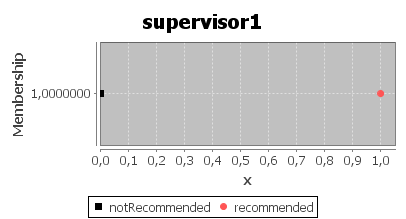
\includegraphics[width=0.6\linewidth]{4_fuzzy-sets-supervisor}
		\caption[Supervisor singleton fuzzy sets]{Supervisor singleton fuzzy sets}
		\label{fig:fs-super}
	\end{figure}

\item \textbf{Solution1}, \textbf{Solution2}, …, \textbf{Solution9}. These variables cover the 9 solutions proposed to reduce communication problems, where each solution shows a series of recommendations and communication means related to user input values (see Appendix \ref{cap:annexB} for a detailed explanation of these solutions). All of them are represented by singleton sets with COGS as defuzzification method (see Figure \ref{fig:fs-solution}). Also note how the proposed communication solution offered as output will be always unique. 
\end{itemize}

	\begin{figure}
		\centering
		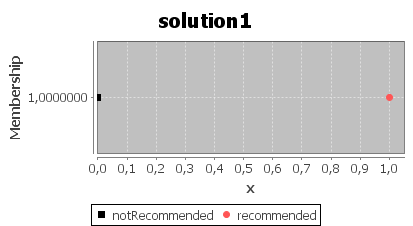
\includegraphics[width=0.6\linewidth]{4_fuzzy-sets-solution}
		\caption[Solutions singleton fuzzy sets]{Solutions singleton fuzzy sets}
		\label{fig:fs-solution}
	\end{figure}

Note how these boolean output variables have been represented by singleton sets where 0 expresses  "not recommended" and 1, "recommended". According to its definition, a fuzzy singleton set is the one whose support is a single point $x$ such that $\mu_a(x) = 1$. In this case, two singleton sets are used, representing the previously mentioned values.

With the input and output variables defined, using jFuzzyLogic for the implementation was not difficult after learning how to use it together with FCL. In general, the system is divided into four distinct parts:

\begin{itemize}
\item First, we have the variable declaration block, as shown in Listing \ref{lst:variables}, where we indicate the input and output variables of the system.

\begin{lstlisting}[caption={[Variables declaration]Variables declaration}, label=lst:variables]
VAR_INPUT
	culturalDist : REAL;
	overlap : REAL;
	age1 : REAL;
	age2 : REAL;
	englishLevel : REAL;
	experience1 : REAL;
	experience2 : REAL;
END_VAR

VAR_OUTPUT
	mediator : REAL;
	training : REAL;
	supervisor1 : REAL;
	supervisor2 : REAL;
	solution1 : REAL;
	solution2 : REAL;
	solution3 : REAL;
	solution4 : REAL;
	solution5 : REAL;
	solution6 : REAL;
	solution7 : REAL;
	solution8 : REAL;
	solution9 : REAL;
END_VAR
\end{lstlisting}

\item Next is the definition block for fuzzy sets, or fuzzification block, where the input values are translated into fuzzy labels (Listing \ref{lst:fuzzification}).

\begin{lstlisting}[caption={[Fuzzification block]Fuzzification block}, label=lst:fuzzification]
FUZZIFY culturalDist // Cultural distance
	TERM veryLow := trape 0 0 0.1 0.3;
	TERM low := trian 0.1 0.3 0.5;
	TERM medium := trian 0.3 0.5 0.7;
	TERM high := trian 0.5 0.7 0.9;
	TERM veryHigh := trape 0.7 0.9 1 1;
END_FUZZIFY

FUZZIFY overlap // Time overlap
	TERM veryLow := trape 0 0 0.1 0.3;
	TERM low := trian 0.1 0.3 0.5;
	TERM medium := trian 0.3 0.5 0.7;
	TERM high := trian 0.5 0.7 0.9;
	TERM veryHigh := trape 0.7 0.9 1 1;
END_FUZZIFY

FUZZIFY age1 // User1's age
	TERM low := trian 16 16 36;
	TERM medium := trian 26 36 50;
	TERM high := trian 40 67 67;
END_FUZZIFY

FUZZIFY age2 // User2's age
	TERM low := trian 16 16 36;
	TERM medium := trian 26 36 50;
	TERM high := trian 40 67 67;
END_FUZZIFY

FUZZIFY englishLevel // English level
	TERM veryLow := trape 0 0 0.1 0.3;
	TERM low := trian 0.1 0.3 0.5;
	TERM medium := trian 0.3 0.5 0.7;
	TERM high := trian 0.5 0.7 0.9;
	TERM veryHigh := trape 0.7 0.9 1 1;
END_FUZZIFY

FUZZIFY experience1 // Experience of user1
	TERM veryLow := trape 0 0 0.1 0.3;
	TERM low := trian 0.1 0.3 0.5;
	TERM medium := trian 0.3 0.5 0.7;
	TERM high := trian 0.5 0.7 0.9;
	TERM veryHigh := trape 0.7 0.9 1 1;
END_FUZZIFY

FUZZIFY experience2 // Experience of user2
	TERM veryLow := trape 0 0 0.1 0.3;
	TERM low := trian 0.1 0.3 0.5;
	TERM medium := trian 0.3 0.5 0.7;
	TERM high := trian 0.5 0.7 0.9;
	TERM veryHigh := trape 0.7 0.9 1 1;
END_FUZZIFY
\end{lstlisting}

\vspace{16px}
\item In the same way, the output values are defined in the defuzzification block (Listing \ref{lst:defuzzification}), following an inverse process to the preceding one.

\newpage 

\begin{lstlisting}[caption={[Defuzzification block]Defuzzification block}, label=lst:defuzzification]
DEFUZZIFY mediator // Communication mediator
	TERM notRecommended := 0;
	TERM recommended := 1;
	METHOD : COGS;
	DEFAULT := 0;
END_DEFUZZIFY

DEFUZZIFY training // Communication training
	TERM notRecommended := 0;
	TERM recommended := 1;
	METHOD : COGS;
	DEFAULT := 0;
END_DEFUZZIFY

DEFUZZIFY supervisor1 // Supervisor for user1
	TERM notRecommended := 0;
	TERM recommended := 1;
	METHOD : COGS;
	DEFAULT := 0;
END_DEFUZZIFY

DEFUZZIFY supervisor2 // Supervisor for user2
	TERM notRecommended := 0;
	TERM recommended := 1;
	METHOD : COGS;
	DEFAULT := 0;
END_DEFUZZIFY

DEFUZZIFY solution1
	TERM notRecommended := 0;
	TERM recommended := 1;
	METHOD : COGS;
	DEFAULT := 0;
END_DEFUZZIFY

DEFUZZIFY solution2
	TERM notRecommended := 0;
	TERM recommended := 1;
	METHOD : COGS;
	DEFAULT := 0;
END_DEFUZZIFY

DEFUZZIFY solution3
	TERM notRecommended := 0;
	TERM recommended := 1;
	METHOD : COGS;
	DEFAULT := 0;
END_DEFUZZIFY

DEFUZZIFY solution4
	TERM notRecommended := 0;
	TERM recommended := 1;
	METHOD : COGS;
	DEFAULT := 0;
END_DEFUZZIFY

DEFUZZIFY solution5
	TERM notRecommended := 0;
	TERM recommended := 1;
	METHOD : COGS;
	DEFAULT := 0;
END_DEFUZZIFY

DEFUZZIFY solution6
	TERM notRecommended := 0;
	TERM recommended := 1;
	METHOD : COGS;
	DEFAULT := 0;
END_DEFUZZIFY

DEFUZZIFY solution7
	TERM notRecommended := 0;
	TERM recommended := 1;
	METHOD : COGS;
	DEFAULT := 0;
END_DEFUZZIFY

DEFUZZIFY solution8
	TERM notRecommended := 0;
	TERM recommended := 1;
	METHOD : COGS;
	DEFAULT := 0;
END_DEFUZZIFY

DEFUZZIFY solution9
	TERM notRecommended := 0;
	TERM recommended := 1;
	METHOD : COGS;
	DEFAULT := 0;
END_DEFUZZIFY
\end{lstlisting}

\vspace{16px}
\item As we have already defined the input and output variables, as well as the fuzzification and defuzzification functions, all that remains is to display the set of rules used by the system, shown in Table \ref{tb:recommender-rules}.

\begin{table}[htb]
	\centering
	\caption{Recommender system rules set}
	\label{tb:recommender-rules}
	\resizebox{\textwidth}{!}{%
	\begin{tabular}{|c|l|}
	\hline
	\textbf{N} &
	  \multicolumn{1}{c|}{\textbf{FCL RULE}} \\ \hline\hline
	1 &
	  \begin{tabular}[c]{@{}l@{}}IF (age1 IS   high OR age2 IS high) AND (overlap IS low OR overlap IS veryLow)  \\ AND  (englishLevel is low OR englishLevel is veryLow) THEN solution1 IS   recommended;\end{tabular} \\ \hline
	2 &
	  \begin{tabular}[c]{@{}l@{}}IF (age1 IS   high OR age2 IS high) AND (overlap IS low OR overlap IS veryLow)\\ AND   (englishLevel is medium) THEN solution2 IS recommended;\end{tabular} \\ \hline
	3 &
	  \begin{tabular}[c]{@{}l@{}}IF (age1 IS   high OR age2 IS high) AND (overlap IS low OR overlap IS veryLow)\\ AND   (englishLevel is high OR englishLevel is veryHigh) THEN solution3 IS   recommended;\end{tabular} \\ \hline
	4 &
	  \begin{tabular}[c]{@{}l@{}}IF (age1 IS   high OR age2 IS high) AND (overlap IS medium OR overlap IS high OR overlap is   veryHigh)\\ AND (englishLevel IS veryHigh OR englishLevel IS high OR   englishLevel IS medium) THEN solution4 IS recommended;\end{tabular} \\ \hline
	5 &
	  \begin{tabular}[c]{@{}l@{}}IF (age1 IS   high OR age2 IS high) AND (overlap IS medium OR overlap IS high OR overlap is   veryHigh)\\ AND (englishLevel IS veryLow OR englishLevel IS low) THEN solution5   IS recommended;\end{tabular} \\ \hline
	6 &
	  \begin{tabular}[c]{@{}l@{}}IF (age1 IS   low OR age1 IS medium) AND (age2 IS low OR age2 IS medium)\\ AND (overlap IS   low OR overlap IS veryLow) AND (englishLevel IS medium OR englishLevel IS   high OR englishLevel IS veryHigh) \\ THEN solution6 IS recommended;\end{tabular} \\ \hline
	7 &
	  \begin{tabular}[c]{@{}l@{}}IF (age1 IS   low OR age1 IS medium) AND (age2 IS low OR age2 IS medium)\\ AND (overlap IS   low OR overlap IS veryLow) AND (englishLevel IS low OR englishLevel IS   veryLow) \\ THEN solution7 IS recommended;\end{tabular} \\ \hline
	8 &
	  \begin{tabular}[c]{@{}l@{}}IF (age1 IS   low OR age1 IS medium) AND (age2 IS low OR age2 IS medium)\\ AND (overlap IS   medium OR overlap IS high OR overlap IS veryHigh)\\ AND (englishLevel IS   veryHigh OR englishLevel IS high OR englishLevel IS medium) THEN solution8 IS   recommended;\end{tabular} \\ \hline
	9 &
	  \begin{tabular}[c]{@{}l@{}}IF (age1 IS   low OR age1 IS medium) AND (age2 IS low OR age2 IS medium) \\ AND (overlap IS   medium OR overlap IS high OR overlap IS veryHigh)\\ AND (englishLevel IS   veryLow OR englishLevel IS low) THEN solution9 IS recommended;\end{tabular} \\ \hline
	10 &
	  IF   (culturalDist IS veryHigh) THEN mediator IS recommended; \\ \hline
	11 &
	  IF   (culturalDist IS high) THEN training IS recommended; \\ \hline
	12 &
	  IF   (experience1 IS low OR experience1 IS veryLow) THEN supervisor1 IS   recommended; \\ \hline
	13 &
	  IF (experience2   IS low OR experience2 IS veryLow) THEN supervisor2 IS recommended; \\ \hline
	\end{tabular}%
	}
\end{table}	

\end{itemize}

Once the system was implemented and ready to be used, it was integrated into the FENCE interface.

\subsubsection{EXPERT SYSTEM INTERFACE}

The integration of the expert system with the FENCE interface is quite simple and easy to use. When the user accesses the "Recommendations" window (shown in Figure \ref{fig:recommendations}), the first thing that will be loaded will be the last recommendations generated for the project selected in the dropdown menu. However, if the user wants to recalculate these recommendations to get an up-to-date list, then simply pressing the "Update" button will display the new list of advices.

	\begin{figure}
		\centering
		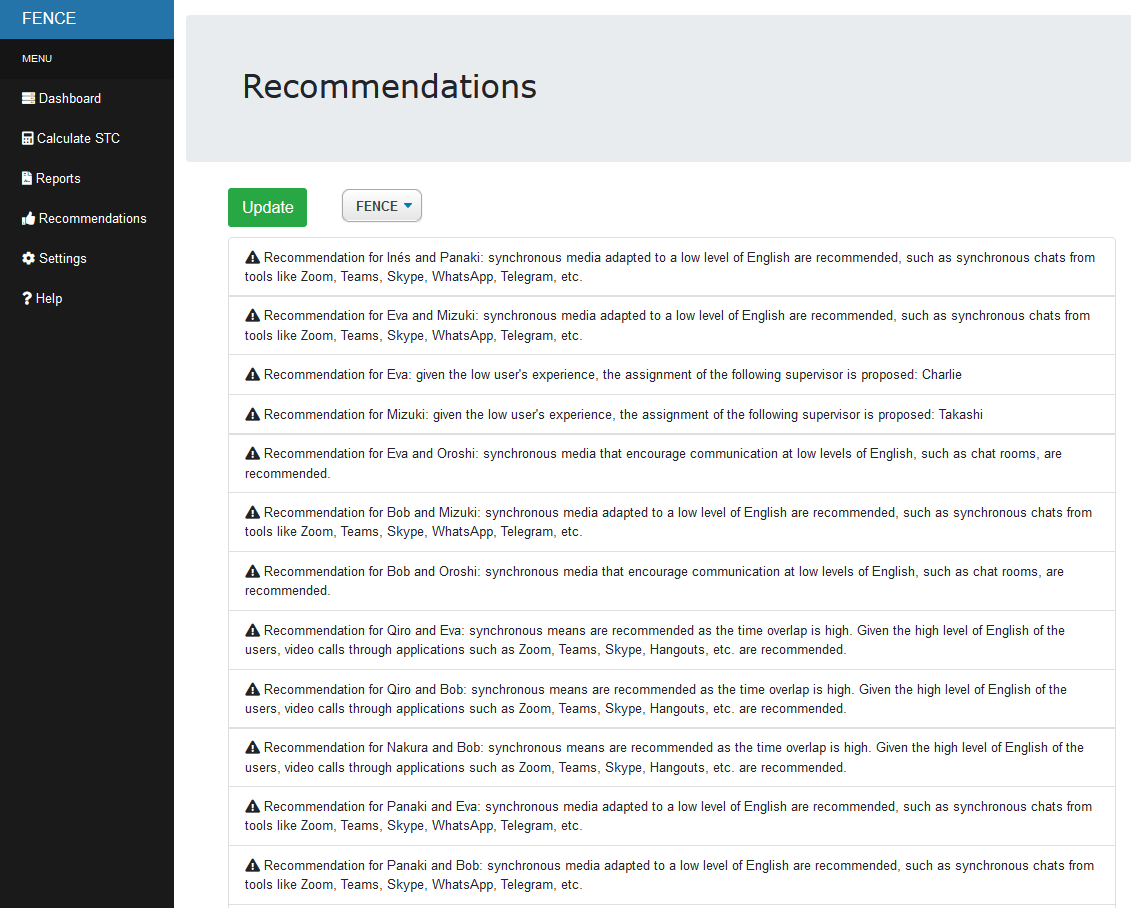
\includegraphics[width=0.9\linewidth]{4_recommendations-window}
		\caption[Recommendations window]{Recommendations window}
		\label{fig:recommendations}
	\end{figure}

As indicated at the beginning of this section, whether or not to show recommendations for certain users should depend on the weight of the coordination gap present among them in the $C_G$ matrix. On this basis, one of the improvements proposed at the end of this phase was the possibility of customizing from which weight in $C_G$ the system would show recommendations for pairs of employees. This feature as well as others related to customization will be covered in the following section.

\subsection{Module 6. Settings and preferences}

The last functional module of FENCE is the one related to customization and settings. The objectives of this module include enabling the user to modify certain parameters used by the tool so that it can be adjusted to particular projects, teams or user’s needs.

After the development of the STC measurement and recommendation modules, it was agreed that the following customisable features may be implemented:

\begin{itemize}
\item On the one hand, the possibility to generally adjust the weight in the $C_G$ matrix considered to provide recommendations between pairs of users. As already explained, when offering recommendations by the expert system, the weight of the cells in $C_G$ matrix is taken as a reference to evaluate if there are communication problems between users and, therefore, to know if it is necessary to recommend communication solutions.

\item On the other hand, it was also considered the possibility of establishing custom thresholds for the $C_G$ weights used to provide recommendations among specific employees. To better illustrate the customization of this $C_G$ weight threshold, let us consider the following example:\newline


\indent\emph{Suppose that the system provides recommendations for any pair of users with a weight in the $C_G$ matrix equal to or greater than 0.4.\newline}

\indent\emph{Two users, Alice and Bob, have a lack of coordination reflected in the $C_G$ matrix with a value of 0.6, which means that the expert system will offer recommendations to improve their communication.\newline}

\indent\emph{However, we know that the communication between Alice and Bob is simple and effective because they are used to working together, so it would be convenient to be able to adjust the $C_G$ threshold value to avoid getting unnecessary recommendations, for example, to 0.9.\newline}

\indent\emph{Thus, the user can set the minimum weight required to receive recommendations for the particular case of Alice and Bob to 0.9 through the FENCE settings interface.\newline}


\end{itemize}

With these ideas in mind, the development of these customizations was conducted (see Figure \ref{fig:settings}). In turn, the option to restore all weights to the established default value was also included, as well as the possibility of establishing these weights at project level, thus increasing customization and flexibility.

\begin{figure}
	\centering
	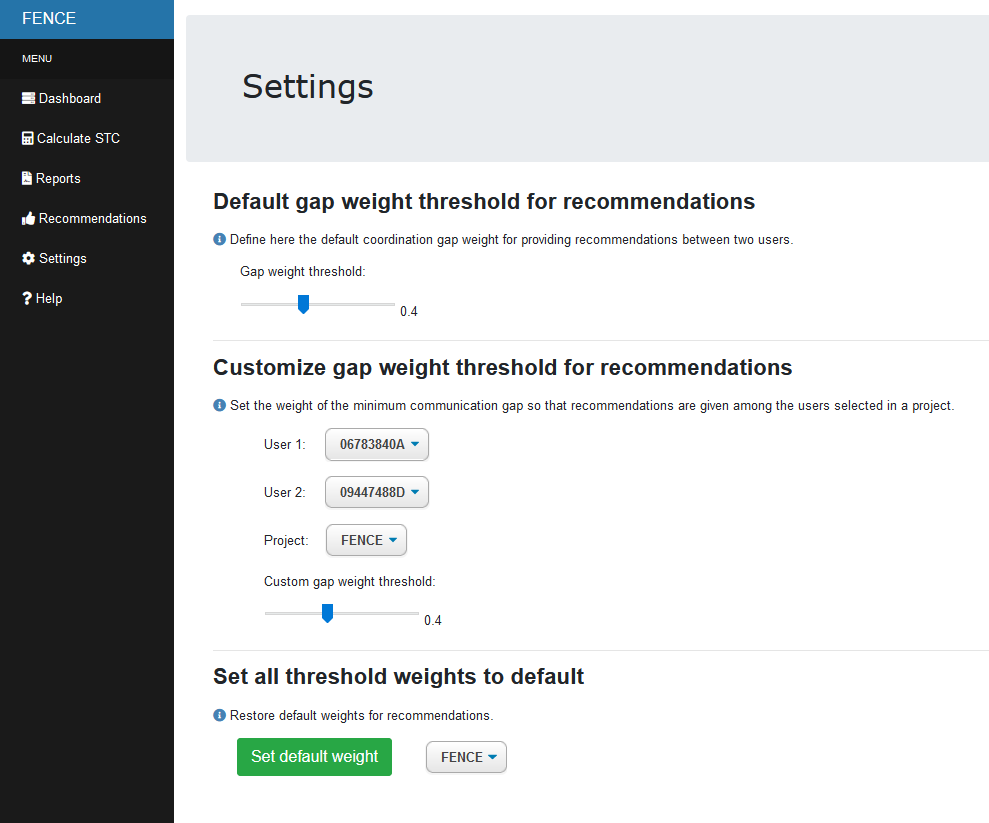
\includegraphics[width=0.9\linewidth]{4_settings-window}
	\caption[Settings window]{Settings window}
	\label{fig:settings}
\end{figure}

In this way, the main functionalities of FENCE had finally been completed. All that remained to be done was to test and make improvements in the presentation and performance of FENCE, an iterative procedure based on stakeholders' feedback.

\section{Transition phase}

Although the tool was already functional and ready to be used, there were still some non-functional changes and actions to be performed. This transition stage includes the performance, usability and optimization testing of FENCE, as well as the deployment of the tool. This actions will be explained in the following subsections.

\subsection{Interface improvements}

With the backend part completed, efforts were focused on improving the application's interface and usability. This work involved reorganizing and improving the cascade style sheets (CSS), optimizing the JavaScript code and improving the overall appearance by modifying the HTML views.

Further graphic information, such as icons and coloured buttons, was also included, as well as a “Help” tab with information about STC and the use of FENCE for its proper management.

\subsection{Algorithms optimization and bug resolution}

Bugs related to the expert system and the recommendations provided were resolved, as well as attempts were made to further optimize the STC measurement algorithms.

Moreover, security improvements were attempted to be added in order to increase the robustness of the tool, such as input control in the database. However, given the time constraints of the project, this aspect was not addressed as deeply as would have been desired, so it is proposed as a future improvement of the tool.

\subsection{First release and documentation}

Once the tool was finally considered to be completed, the building and packaging of the distributable executable of FENCE was performed. At the same time, most of the tool's documentation was produced in this phase: both in the GitHub repository where it is hosted and in this document itself.

\subsection{Application deployment}

Finally, the application was deployed on the Heroku cloud platform. This platform as a service (PaaS) allows free and limited deployment of cloud services, serving as an example of how FENCE would be used in a real web environment (see Figure \ref{fig:heroku-app}, where the service hosted on \url{www.fenceapp.herokuapp.com} is shown).
	
	\begin{figure}
		\centering
		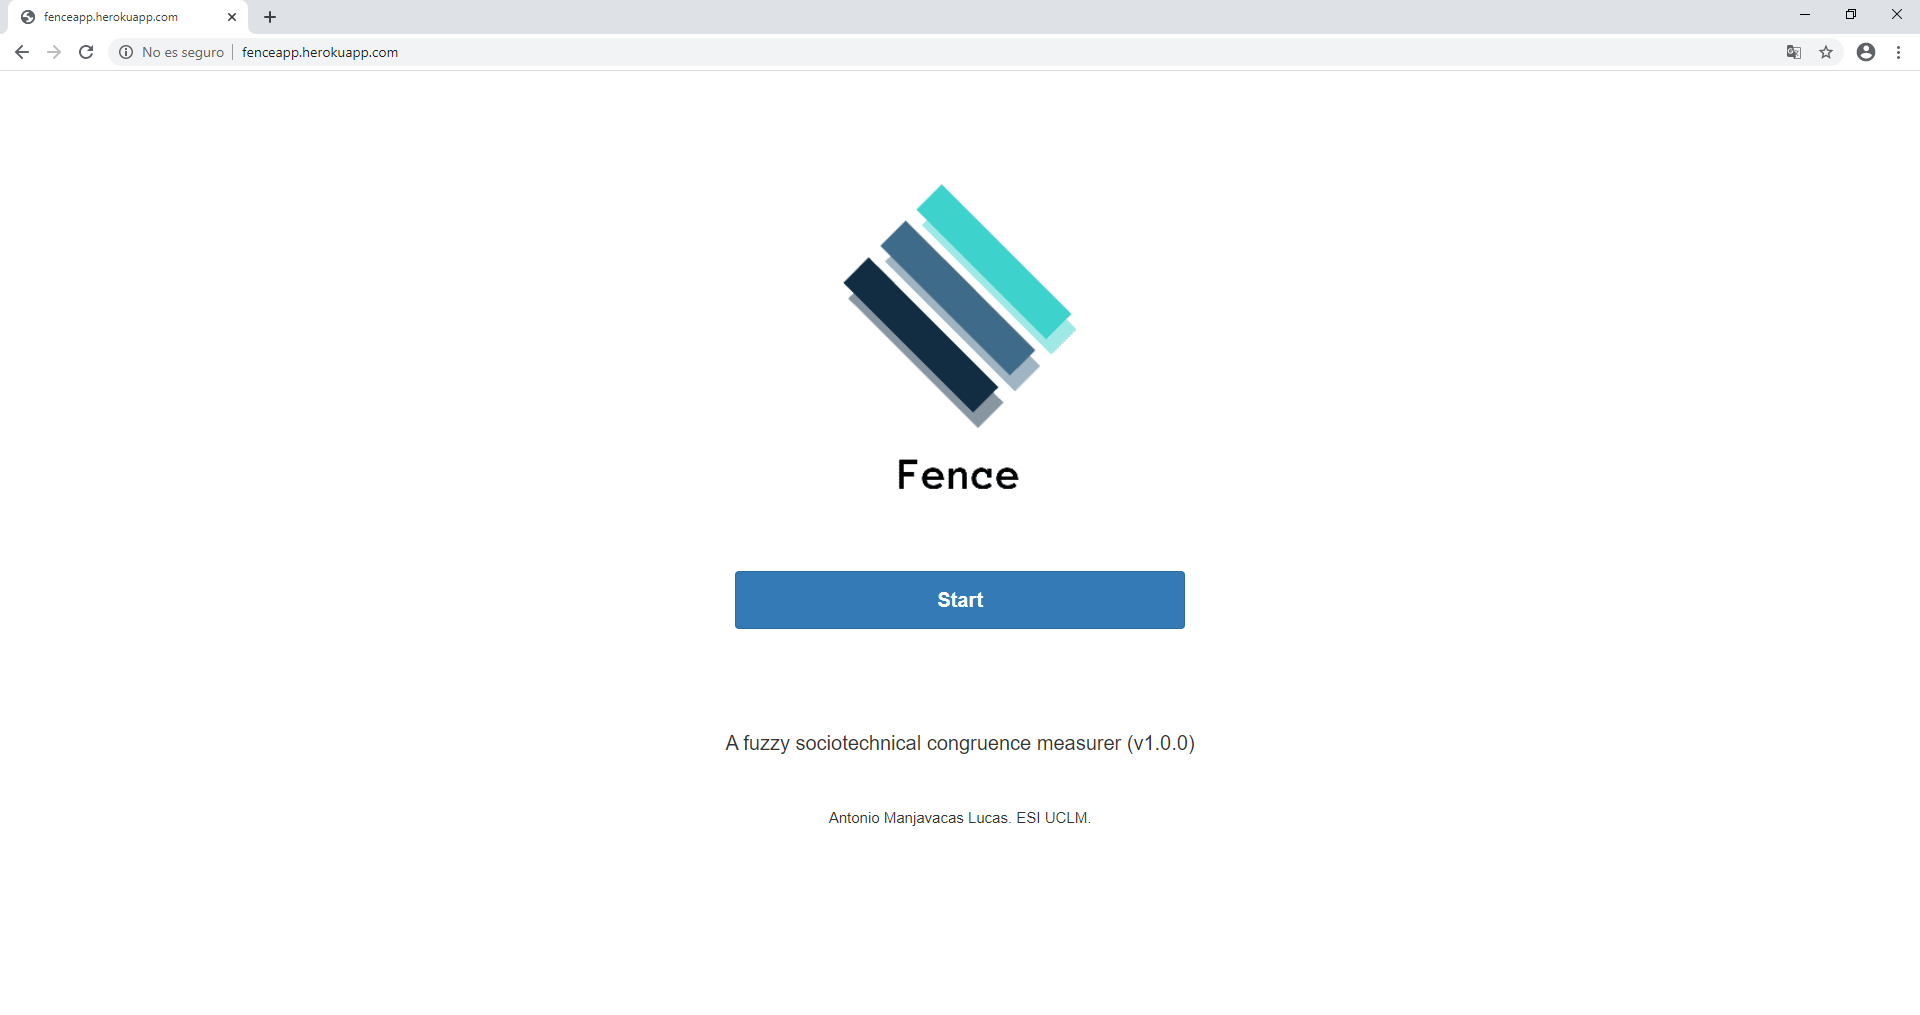
\includegraphics[width=0.9\linewidth]{4_heroku-app}
		\caption[FENCE deployed in Heroku]{FENCE deployed in Heroku Cloud Platform}
		\label{fig:heroku-app}
	\end{figure}

It should also be noted that FENCE was initially considered as a tool for local use, and that it would be necessary to include security and access policies to ensure its concurrent use by multiple users. However, it can be seen that in this first version it is completely operative on the web, and that it would be a matter of future improvements to better adapt the tool to a fully distributed environment.